% Activate the following line by filling in the right side. If for example the name of the root file is Main.tex, write
% "...root = Main.tex" if the chapter file is in the same directory, and "...root = ../Main.tex" if the chapter is in a subdirectory.
 
%!TEX root =  

\chapter[Monte Carlo Simulation]{Monte Carlo Simulation Events}

In order to understand both the signal and backgrounds better, Monte Carlo (MC) simulation datasets are computer-
generated simulation events that allow a physicist to develop and validate an analysis.  The generation and refinement of MC 
algorithms and datasets could be a thesis in its own right, but this section will touch on some of 
the most relevant features of the MC datasets used in this analysis.


\section{MC Creation Procedure}
\label{sec:mc-gen-overview}
MC events are generally created in four major steps.  
\begin{enumerate}
    \item First, the generator uses quantum field theory to simulate the hard 
    scatter, generally starting with a proton and ending with all final-state particles.  
    \item Then those particles are handed off to a dedicated algorithm that simulates 
    how they would shower and hadronize, where appropriate.  
    \item Next, the resulting particles from the first two steps are put 
    into a detector simulation, which uses information on the detector materials and geometry 
    to understand how the particles evolve as they travel through the ATLAS detector.  
    \item The detector's response to the particles is simulated in a 
    digitization and reconstruction step, so that the final output is an event that 
    has characteristics similar to those of a ``real'' event of that type in the ATLAS detector. 
\end{enumerate} 

\section{Signal Monte Carlo Simulations}
MadGraph 5 \cite{MadGraph} is used to generate the signal MC simulation events, with showering and 
hadronization done in Pythia6 \cite{Pythia6}.  The generation process uses a 5 flavor scheme PDF 
(parton distribution function), meaning that MadGraph models $b$-quarks in the proton as 
well as the more common light flavor (up, down, charm and strange quarks, 
and gluons).  In addition to the Higgs production with the associated $b$-quark and 
the Higgs decay, there can also be extra jets in the event from initial state radiation (ISR) 
and/or final state radiation (FSR).  We allow up to two additional partons per 
event in the signal MC simulations\footnote{this statement refers to extra partons being
generated at the level of the Feynman diagrams; the later hadronization and parton showering step can generate additional
partons in the final state and events must be matched to the hard scatter diagrams to avoid double-counting}; 
the cross-section calculations tend to be more 
accurate for higher numbers of extra partons allowed (again, at the Feynman diagram level), 
but at the cost of exponentially slower 
generation times (Table~\ref{tab:mg_times}).  We found two additional partons to be a reasonable cutoff where the kinematic
distributions and cross section calculations were only minimally 
affected by allowing for higher numbers of extra partons, but the generation 
time was still acceptably quick.  The matching scale for knitting together the hard scatter
calculations in MadGraph with the Pythia hadronization and showering was set to 20 GeV.

%--------------------------------------------------------
\begin{table}
   \caption{The cross sections and generation times for MadGraph signal MC simulations as a function
   of number of additional partons allowed, for 0-3 partons.  There is approx. 2.5\%
   difference between the 2-parton and 3-parton cross sections, which comes at a cost
   of hours of CPU time per batch of 10,000 events.  The times quoted here are for generating 10,000 events per 
   sample, before hadronization.  The generation process imposes a $p_T$ cut of 5 GeV on all jets,
   no further $p_T$ cut on $b$-jets, a minimum $dR$ of 0.4 between jets (no minimum between
   $b$-jets), and a maximum $|\eta|$ of 5.0. \label{tab:mg_times}} 
    \center
    \begin{tabular}{ c c c } \hline\hline
    Process & $\sigma [pb]$ & time \\ \hline
    $pp\rightarrow h^0b + \leq 0j$ & 1.843e-5 $\pm$ 4.2e-08 & seconds \\
    $pp\rightarrow h^0b + \leq 1j$ & 2.555e-5 $\pm$ 7.3e-08 & seconds \\
    $pp\rightarrow h^0b + \leq 2j$ & 2.762e-5 $\pm$ 8.2e-08 & minutes \\
    $pp\rightarrow h^0b + \leq 3j$ & 2.83e-5 $\pm$ 9e-08 & $~$ 4 hours \\  \hline
    \end{tabular}
\end{table}

%--------------------------------------------------------



%--------------------------------------------------------
\begin{table}
   \caption{The signal MC samples and their parameters. These widths were generated with 
   a $\tan\beta$ value of 30.  The dataset ID is a reference for internal ATLAS bookkeeping.\label{tab:sig_mc_parameters} }
    \center
    \begin{tabular}{ c c c } \hline\hline
    Dataset ID & physical mass (GeV) & width (GeV) \\ \hline
    181120     & 250        & 1.68682 \\
    181121     & 280        & 1.92318 \\
    181122     & 310        & 2.50849 \\
    181123     & 350        & 3.23507 \\
    181124     & 400        & 3.93561 \\
    181125     & 450        & 4.71906 \\
    181126     & 500        & 5.59454 \\
    181127     & 550        & 6.84368 \\
    181128     & 600        & 8.11044 \\
    181129     & 650        & 9.26688 \\
    181130     & 700        & 10.3760 \\
    181131     & 800        & 12.5049 \\ \hline
    \end{tabular}
\end{table}

%--------------------------------------------------------




The Madgraph signal generation is done for 12 different mass points, spanning physical
Higgs masses of 250-800 GeV. 
Below 250 GeV, the daughter $b$-jets from the Higgs tend to be 
too low-$p_T$ to fire the trigger, while above 800 GeV it would require very 
high values of $\tan\beta$, above 60, to have a signal cross section large enough
for experimental detection in this analysis, and perturbativity starts to break
down for such large values of $\tan\beta$.
Since both the production and decay of $bH\rightarrow b\bar{b}b$ 
happen via SM interactions, with SUSY only becoming relevant for increasing the production cross section and 
widening the intrinsic width of the $A/H$ distributions, the signal generation can 
be done by using an SM $bH\rightarrow b\bar{b}b$ production model but with a 
modified $Hb\bar{b}$ coupling and Higgs width.  There are 300,000 signal events generated for each mass point.

% ATF-II source: http://iopscience.iop.org/1742-6596/396/2/022031
The detector simulation for the signal MC was done using AtlFast-II (AFII) \cite{ATF2}, 
a modified version of Geant4 \cite{Geant4-1, Geant4-2} designed 
to cut down on the considerable time required for simulating particle interactions with the detector, especially 
showers in the calorimeter.  AFII does full simulation of the inner detector and tracking, but 
uses frozen shower shapes taken from a large collection of pre-generated samples to speed up 
the simulation.  After simulation, the digitization and reconstruction are handled by the ATLAS standard algorithms 
in the ATHENA framework, as is standard for all ATLAS MC.    



%https://indico.cern.ch/event/235341/contribution/1/material/slides/0.pdf
\subsection{Generator Comparisons}
In addition to MadGraph, Sherpa and Pythia are some other signal MC generators that 
were studied.  Pythia does not include Feynman diagrams that include extra partons 
in the final state, but instead gets events with additional partons from the showering
that happens after the ``base process'' \footnote{Pythia has the additional disadvantage
that Pythia6 was being phased out by ATLAS as this analysis was starting, and Pythia8 
had not been validated for this signal process or any closely related ones}.  
Sherpa has the disadvantage that
the Higgs is not stored in the truth table, which makes it impossible to positively
disambiguate between Higgs daughter $b$-quarks and associated $b$-quarks.  This is not
a bug per se, but rather reflects the fact that it can be indeterminate on a quantum mechanical level
which $b$-quarks come from the Higgs decay vs. associated production.  However, between
the time that the signal generator studies were conducted and the writing of this thesis,
a patch has been written that records the Higgs in the truth table, and might be 
deployed in future Sherpa releases.  Sherpa
also shows kinematic differences from both MadGraph and Pythia in the $p_T$ of the truth
jets (Figure~\ref{fig:sig_gen_compare}), which of course then also propagates through to the $m_{b\bar{b}}$ distribution
(Figure~\ref{fig:mbb_sherpa_pythia_madgraph}).


\begin{figure}
  \center
  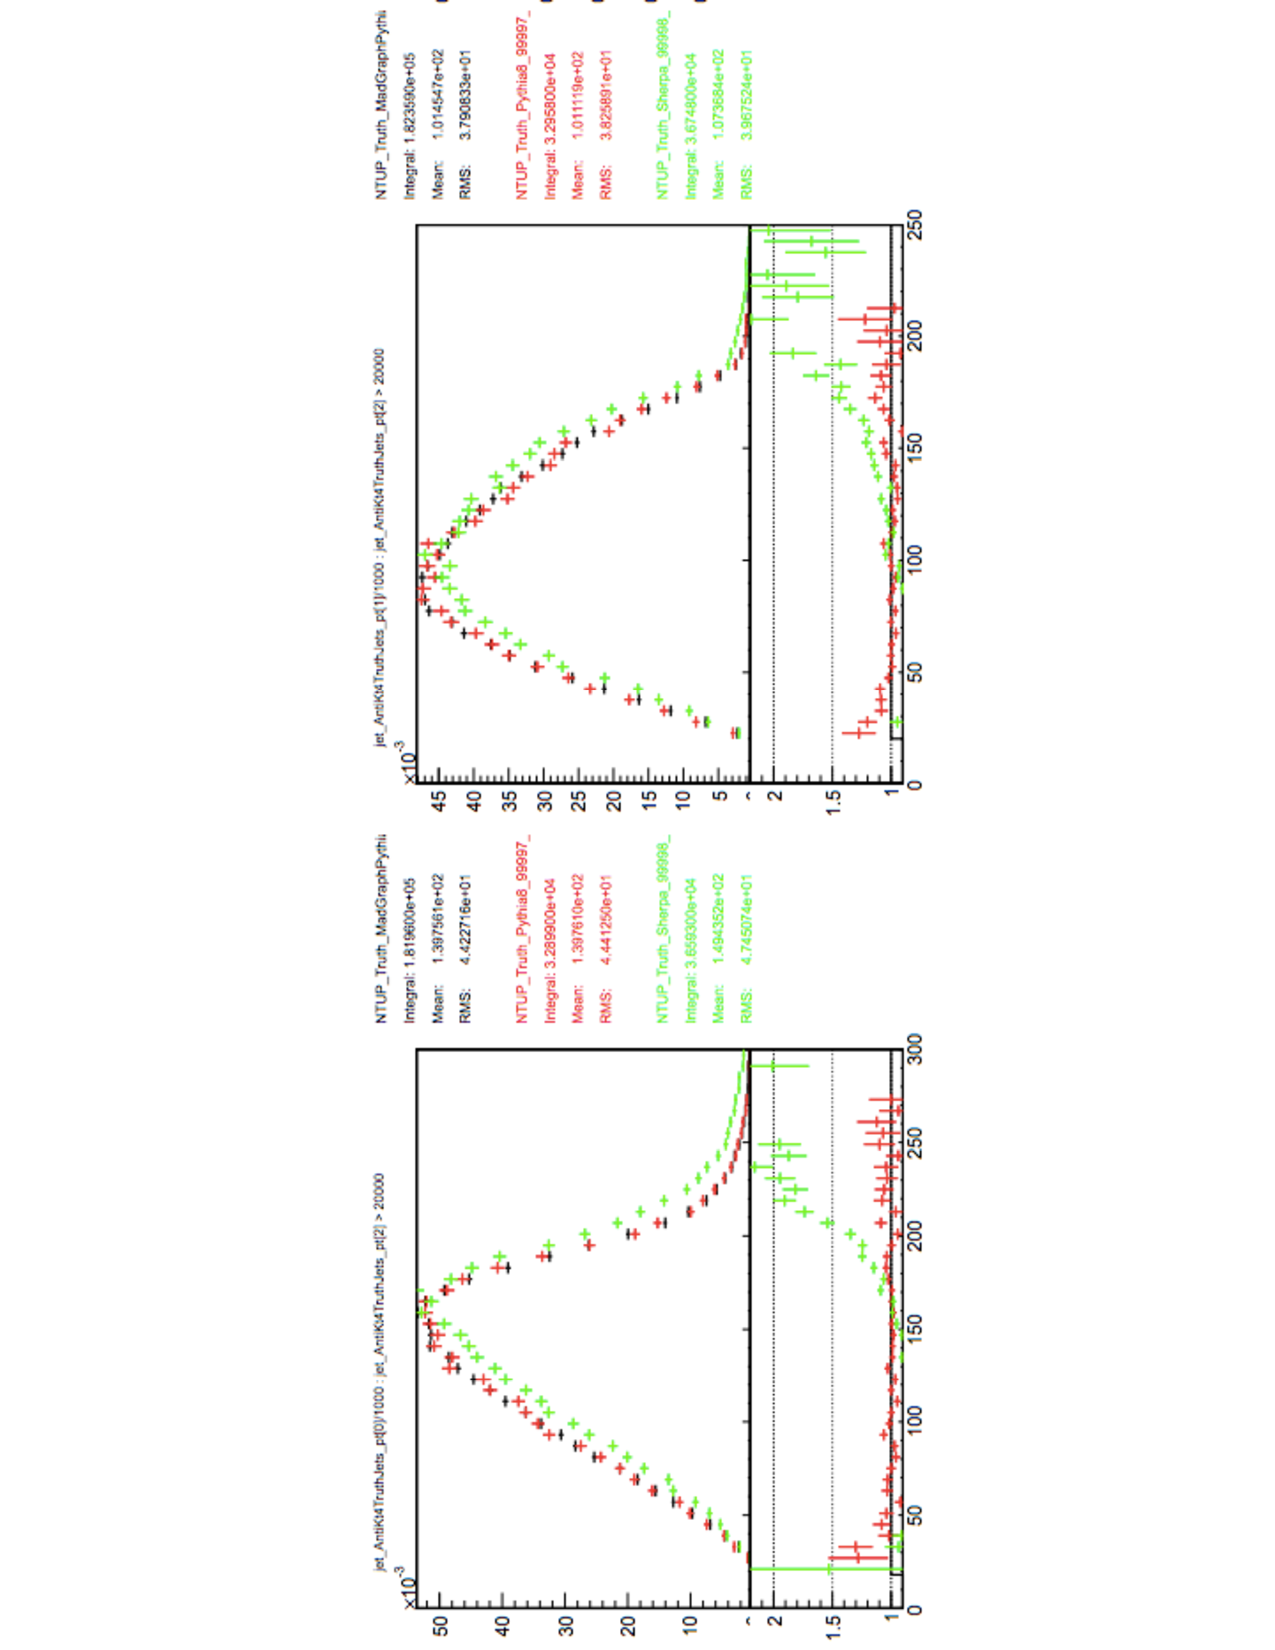
\includegraphics[width=0.7\textwidth, angle=270]{MonteCarlo/figures/sig_gen_compare.pdf}
  \caption{$p_T$ distributions for the leading two jets 
  for Pythia (red), Sherpa (green) and MadGraph (black) for a 
  physical Higgs mass of 380 GeV.  
  Pythia and MadGraph show good agreement, while Sherpa jets are systematically harder.  \label{fig:sig_gen_compare}}
\end{figure}
\begin{figure}
  \center
  \includegraphics[width=0.7\textwidth]{MonteCarlo/figures/mbb_sherpa_pythia_madgraph.pdf}
  \caption{$m_{bb}$ distributions for the leading two jets 
  for Pythia (red), Sherpa (green) and MadGraph (black) for a physical Higgs mass of 380 GeV.  
  Pythia and MadGraph show good agreement, while the Sherpa $m_{bb}$ distribution is higher and more sharply peaked. 
  \label{fig:mbb_sherpa_pythia_madgraph}}
\end{figure}

In order to understand if the disagreement between Sherpa and MadGraph/Pythia 
in the $m_{bb}$ distribution was caused, at least in part, by
mixing up the associated $b$-jets and the Higgs daughter jets, we changed the Sherpa
generation process to $bH\rightarrow b\tau\tau$ and examined the properties of the
Higgs itself in addition to the jets (or $\tau$ leptons) in the event.  The $p_T$ and 
$\eta$ distributions of the di-tau (i.e. Higgs) system are in Figures~\ref{fig:di_tau_pt}
and~\ref{fig:di_tau_eta}, and the $m_{\tau\tau}$ distribution is in Figure~\ref{fig:di_tau_mass}.



\begin{figure}
  \center
  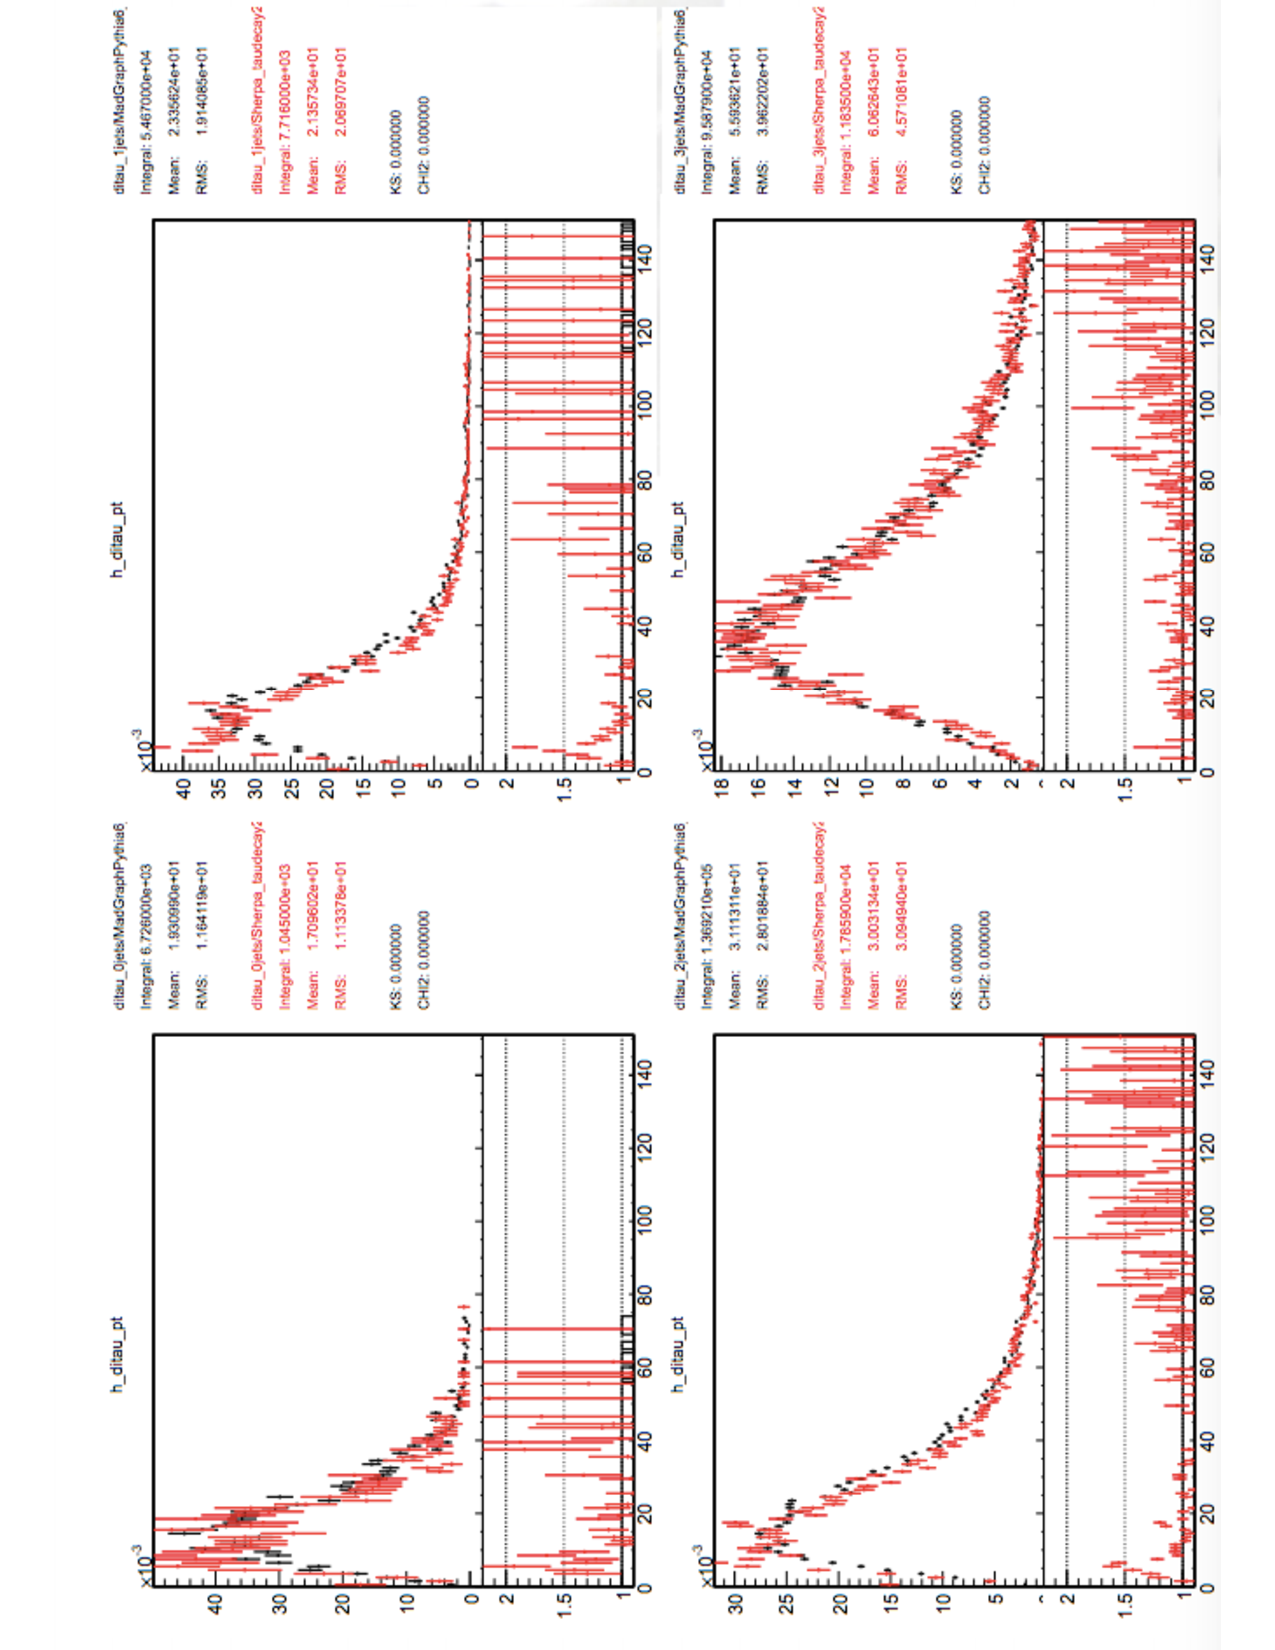
\includegraphics[width=0.8\textwidth, angle=270]{MonteCarlo/figures/di_tau_pt.pdf}
  \caption{$p_T$ distributions for the two $\tau$ leptons (i.e. the Higgs $p_T$) for Sherpa (red) and Madgraph (black) for zero (upper
  left), one (upper right), two (lower left), and three (lower right) additional jets per event. 
  \label{fig:di_tau_pt}}
\end{figure}
\begin{figure}
  \center
  \includegraphics[width=0.8\textwidth, angle=270]{MonteCarlo/figures/di_tau_eta.pdf}
  \caption{$\eta$ distributions for the 2 $\tau$ leptons (i.e. the Higgs $\eta$) for Sherpa (red) and Madgraph (black) for zero (upper
  left), one (upper right), two (lower left), and three (lower right) additional jets per event. 
  The Higgs is more forward (larger $|\eta|$) in Sherpa than in MadGraph.  \label{fig:di_tau_eta}}
\end{figure}
\begin{figure}
  \center
  \includegraphics[width=0.8\textwidth, angle=270]{MonteCarlo/figures/di_tau_mass.pdf}
  \caption{$m_{\tau\tau}$ distributions for the two $\tau$ leptons for Sherpa (red) and Madgraph (black) 
  for a 380 GeV Higgs particle.  Although the agreement is not perfect in the tails of the distribution,
  the agreement is much better than in the $m_{bb}$ distributions, suggesting that the challenges
  of correctly identifying the Higgs daughters in Sherpa is a major factor. 
  \label{fig:di_tau_mass}}
\end{figure}


Upon more careful examination, we found that Sherpa would fail with a segmentation fault
when trying to produce 
$gg\rightarrow H$ Feynman diagrams, and so those diagrams had been excluded from
the initial production, although
an exchange with the Sherpa authors\footnote{most notably Stefan H\"{o}che and Steffen 
Schumann, who we thank for their helpful advice throughout this analysis} provided 
a patch that enabled $gg\rightarrow H$ diagrams.  To understand
if the absence of $gg\rightarrow H$ diagrams in Sherpa was responsible for the disagreement
with MadGraph, we generated samples of MadGraph events with and without the $gg\rightarrow H$
diagrams and compared the $p_T$ and $\eta$ of the Higgs system (Figure ~\ref{fig:ggH}).
The Higgs $p_T$ and $\eta$ do not show a bias depending on whether the gluon diagrams
are included or not, so it is not clear that including the gluon diagrams in Sherpa would
resolve the disagreement that we see. 

\begin{figure}
  \center
  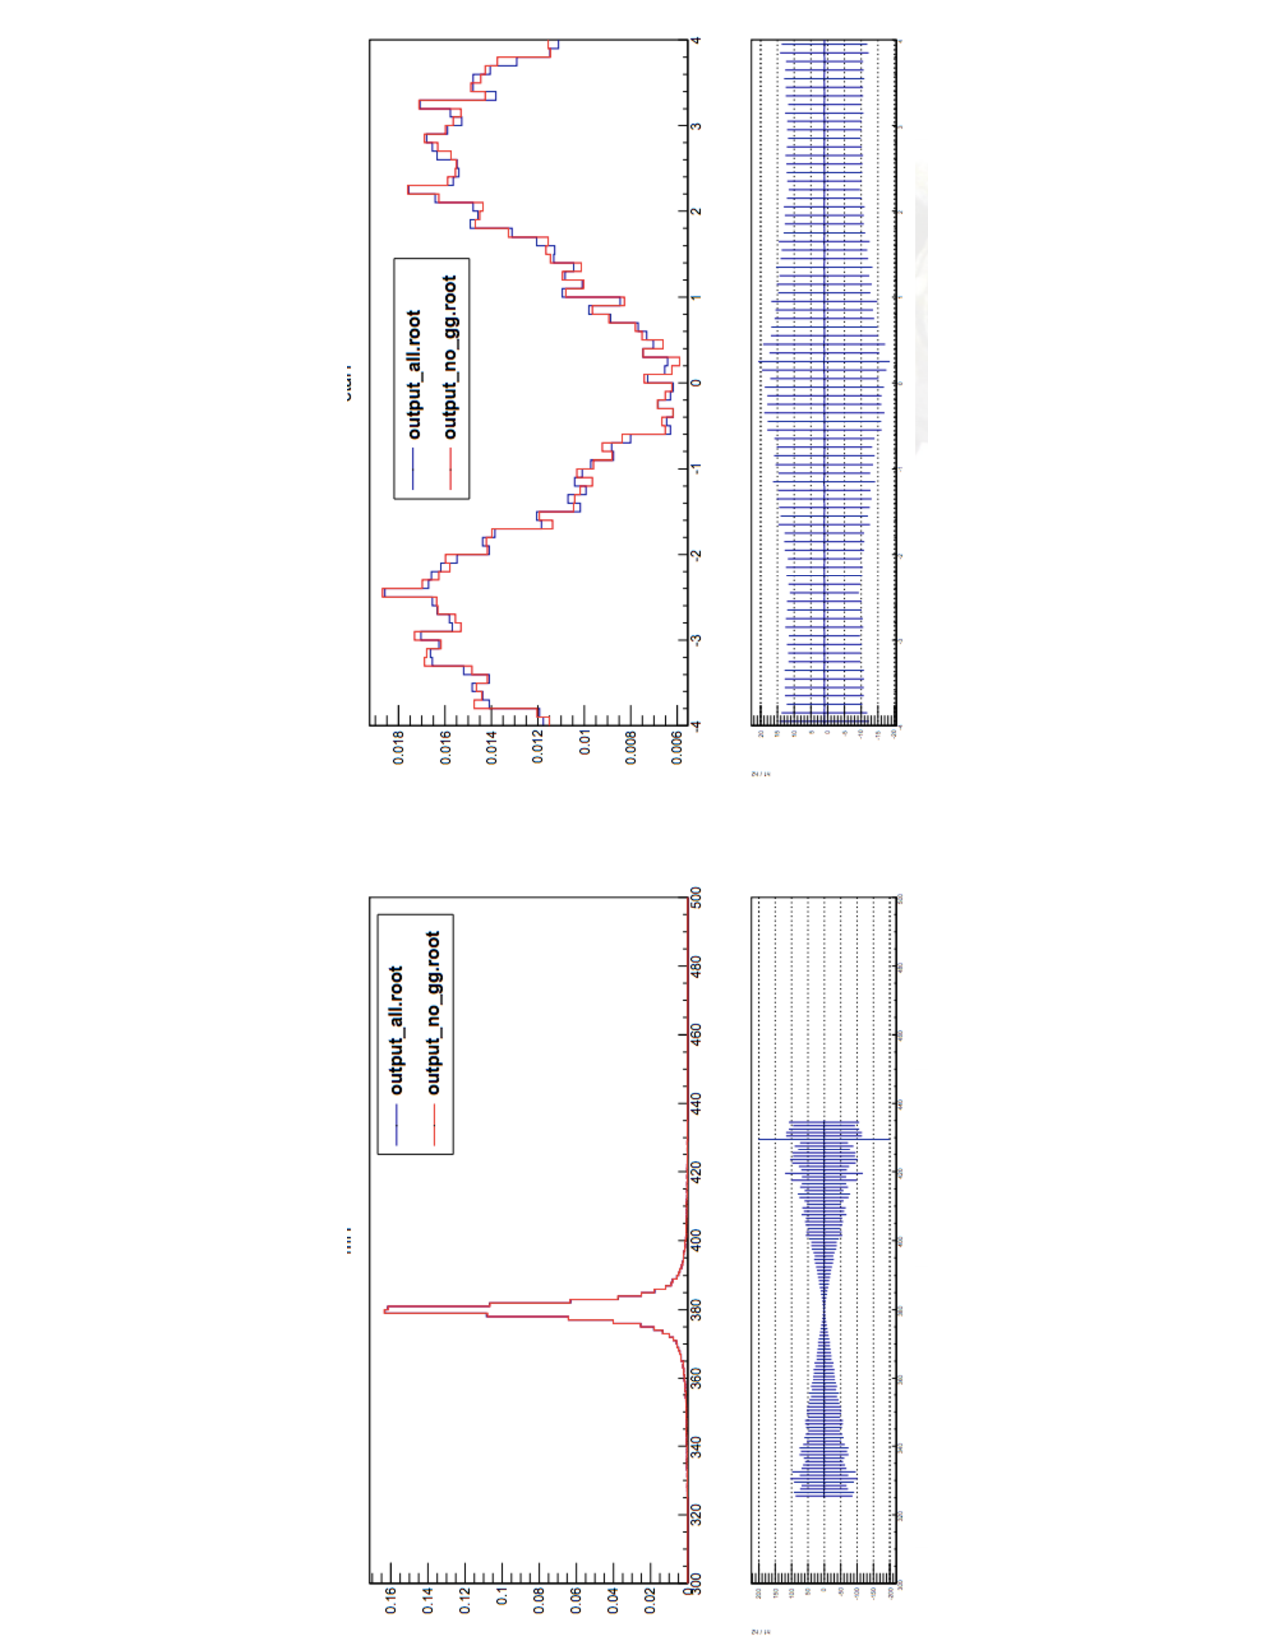
\includegraphics[width=0.8\textwidth, angle=270]{MonteCarlo/figures/ggH.pdf}
  \caption{The $m_{\tau\tau}$ ($m_A$=380 GeV) distribution (left) and $\eta$ of the $\tau$ leptons (right)
  for $bH\rightarrow b\tau\tau$ events in Sherpa,
  with and without gluon fusion diagrams being included.  The ratio plots in the lower part of the
  figures show that the inclusion of the gluon fusion diagrams does not change the kinematics of the
  Higgs and its daughters. 
  \label{fig:ggH}}
\end{figure}

As a result of these studies, we conclude that the likely cause of the Sherpa 
disagreement is ambiguity in the selection of the Higgs daughter $b$-jets, since
the reconstructed Higgs mass agreement between Sherpa and MadGraph improves substantially when looking
at Higgs events decaying to $\tau\tau$ (where the combinatorics are trivial).
MadGraph is also the generator of choice for the $H/A$ searches in the $\tau\tau$ 
decay channel, which makes combinations or comparisons of those searches
more straightforward than it would be if they use different generators.

\section{Background}
\subsection{QCD Background}
Although QCD is the largest and most important background in this analysis, fully modeling 
it with MC simulation has some important drawbacks, which motivates our decision to use a 
mostly data-driven background estimation method.  That having been said, MC can 
still be a very valuable tool for making basic estimates and validating assumptions. 

There are two major types of QCD background in this analysis: first, when 
there is one or more mistakenly $b$-tagged light flavor or charm jets, 
which we call \textit{reducible} because, at least in theory, 
it could be identified and isolated/removed; and second, the \textit{irreducible} 
QCD background in which three real $b$-jets are present in the final 
state but without the intermediate resonance of the Higgs.  Both sources of background are 
expected to be significant but generally require different MC generation strategies.



\subsubsection{QCD Multijet}
The ATLAS QCD multijet MC dataset is generated using Pythia8 \cite{Pythia8}.  
One of the major challenges of a truly inclusive sample like this one is that 
low-$p_T$ jets dominate the production cross section but generally have 
very low efficiency through the triggers or analysis cut flows, which is addressed by 
generating events several times with filtering applied based on the $p_T$ 
of the leading jet.  This leads to a distinctive ``slice'' structure to 
the sample, where 8 different slices are generated, each with a different $p_T$ 
range for the leading jet, and then the slices are knitted together with different 
relative weights to produce an inclusive spectrum with high statistics at all $p_T$ values.  

\begin{table}[h]
 \begin{center}
\caption{Hard subprocesses simulated in the inclusive QCD MC event sample, along with their cross sections. Here
$j=u,\bar{u},d,\bar{d},s,\bar{s},c,\bar{c},g$.  The QCD slices are defined by the $p_T$ cut placed
on the leading jet in the event, which is documented in the ``$p_T$ range'' column.  The dataset
ID is noted as a reference for internal ATLAS bookkeeping.
\label{tab:qcd_mc_parameters}}
    \begin{tabular}{l r r r r r} \hline \hline
    Index & Dataset ID & $p_T$ Range& Cross Section (nb)& Filter Eff   & N Events \\ \hline
    0     &  147910    & 0-20        &  7.285$\times$10$^7$    &   0.98557 & 1000000 \\
    1     &  147911    & 20-80       &  7.285$\times$10$^7$    &   0.00012909 & 999996  \\
    2     &  147912    & 80-200      &  2.6359$\times$10$^4$   &   0.0039901 & 999893 \\
    3     &  147913    & 200-500     &  5.442$\times$10$^2$    &     0.001222 & 914584 \\
    4     &  147914    & 500-1000    &  6.4435                 &   0.00070839 & 999773 \\
    5     &  147915    & 1000-1500   &  3.9739$\times$10$^{-2}$&    0.0021516 & 957565 \\
    6     &  147916    & 1500-2000   &  4.161$\times$10$^{-4}$ &    0.0046773 & 299929 \\
    7     &  147917    & 2000+       &  4.0636$\times$10$^{-5}$&     0.014595 & 299988 \\ \hline
    \end{tabular}
  \end{center}
\end{table}

ATLAS has a high-statistics inclusive QCD MC sample that is used primarily in 
this analysis for understanding the QCD background from 
mistagged charm and light flavor (Table~\ref{tab:qcd_mc_parameters}).  Since 
the sample is inclusive, there is no filtering on the flavor of the jets 
that are produced (although there is dedicated effort to have high-$p_T$ 
jets simulated with adequate statistics) and the vast majority of jets are light or 
charm jets.  As a result, while we use this sample to estimate the 
efficiency and flavor composition of the QCD production in ATLAS as a whole, a 
particularly important background (QCD $b\bar{b}b$) is virtually absent from this sample.


\subsubsection{$b$-Enriched QCD Multijet}
\label{sec:bb_qcd_mc}
Since the inclusive QCD Multijet samples are inadequate for understanding the $b\bar{b}$ and 
$b\bar{b}b$ QCD backgrounds, we generate a dedicated sample that undergoes filtering to 
enrich it in heavy flavor.  This sample is generated using Sherpa 1.4.3 
\cite{Sherpa} and detector simulation is done with AFII.  This sample 
starts with a 5-flavor PDF that assumes massive $b$-quarks and 
2, 3 or 4 final state partons; then a filter is applied that 
requires that the leading 2 partons in the event be true $b$-quarks, 
as well as requiring that the leading parton have a $p_T$ 
of at least 10 GeV and the leading (subleading) jet have a $p_T$ of
130 (45) GeV; additionally, the $b$-hadrons and jets must have $|\eta|<$2.9 
\footnote{These kinematic requirements help keep an acceptable efficiency when 
the sample is passed through the trigger and offline cuts}.  We further enhance
the $b\bar{b}$ contribution to the generation process by setting a flag (called enhance\_factor
in the Sherpa job options) that enhances $g\rightarrow b\bar{b}$ splitting.

A scale factor of 2.07 was applied to the MC to  
reach the same normalization as the full 2012 data (after the trigger and cuts are 
applied).  This scale factor is based on the calculated total cross section and
filter efficiency of the $b\bar{b}$ QCD MC (Table~\ref{tab:sherpa_subprocesses}), as well
as the number of MC events that were generated and the 2012 luminosity. 
In addition, the MC has pileup reweighting and $b$-tagging scale factors
applied.  

%%% START HERE
As is detailed much more thoroughly in Sections~\ref{sec:background_strategy}
and~\ref{sec:n_jets_sig}, the final analysis is categorized by the $b$-tag
status of the third jet in each event, and the number of jets in each event.
The $b$-tag categorization splits the sample based on whether the third jet 
in the event has a third tight-tagged $b$-jet (called the \textit{bbb} category),
a third jet that passes a loose $b$-tag but not a tight one (called \textit{bbloose})
or there is no third $b$-tagged jet present (\textit{bbanti}).  Events are
also categorized based on whether they have three, four, or five or more jets.
%Each of these features has three different categories, so there are nine categories
%overall when performing the final fit and search.  When validating the bb QCD MC sample,
%we categorize the events in the same way (three categories in $b$-tag, and three
%categories in $n_{jets}$) so that we do not miss any kinematic differences 
%that might be category-specific.  

First we check the relative normalization of the nine categories.
The number of weighted MC (data) events in each of the jet and tag
categories can be seen in Table~\ref{tab:bb_qcd_mc_categories}.  The MC
generally underestimates the number of data events in each category,
with the notable exception of the \textit{bbanti} 3-jet category, where 
the data has fewer events than the MC predicts.  The discrepancy is about
3.2\%, but as this category has the highest statistics of any category,
that is still a difference of about 22,000 events.

\begin{table}
    \begin{center}
    \caption{In addition to examining the shapes of the kinematic distributions
    in data vs. in bb QCD MC simulation events, the relative normalization of the different categories
    is computed and compiled.  The data and bb QCD MC events are passed through the analysis
    framework, applying the trigger and cuts, and then a scale factor of 2.07 is applied
    to the bb QCD MC simulations to bring the overall number of events to the same as the number of
    events in data.  Then the bb QCD MC (data) events are categorized by the tag status
    and number of jets in the event. \label{tab:bb_qcd_mc_categories}}
        \begin{tabular}{ c c c c }
                         & 3 jets            & 4 jets            & 5+ jets \\
        \textit{bbb}     & 77,288 (92,853)   & 70,289 (74,060)   & 52,998 (54,753) \\
        \textit{bbloose} & 59,189 (56,826)   & 46,521 (49,502)   & 30,491 (34,725) \\
        \textit{bbanti}  & 693,518 (671,412) & 276,593 (285,076) & 122,354 (128,712) \\
        \end{tabular}
    \end{center}
\end{table}




%---------------------------------------
\begin{table}[h]
 \begin{center}
\caption{Hard subprocesses simulated in the bb QCD MC event sample, along with their cross sections. Here
$j=u,\bar{u},d,\bar{d},s,\bar{s},c,\bar{c},g$}.  Kinematic cuts 
on these samples are detailed in Section~\ref{sec:bb_qcd_mc}.
\label{tab:sherpa_subprocesses}
    \begin{tabular}{l|r} \hline \hline
   subprocess      & cross section (pb)\cr \hline

$jj\rightarrow b\bar{b}jj$ & 58531 \cr
$jj\rightarrow b\bar{b}j$ & 33411 \cr
$bj\rightarrow bjj \ \ +\ \  \bar{b}j\rightarrow \bar{b}jj$ & 22147 \cr
$bj\rightarrow bjjj \ \ +\ \  \bar{b}j\rightarrow \bar{b}jjj$ & 16282 \cr
$bj\rightarrow b j \ \ +\ \  \bar{b} j\rightarrow \bar{b} j$ & 12135 \cr
$jj\rightarrow b\bar{b}$ &  1672 \cr
$cj\rightarrow c b\bar{b}j \ \ +\ \  \bar{c} j\rightarrow \bar{c}  b\bar{b}j$ & 1602 \cr
$bj\rightarrow b b\bar{b}j \ \ +\ \  \bar{b} j\rightarrow \bar{b}  b\bar{b}j$ & 997 \cr
$jj\rightarrow b\bar{b}c\bar{c}$ &  776 \cr
$cj\rightarrow c b\bar{b} \ \ +\ \  \bar{c} j\rightarrow \bar{c}  b\bar{b}$ & 681 \cr
$bj\rightarrow b b\bar{b} \ \ +\ \  \bar{b} j\rightarrow \bar{b}  b\bar{b}$ & 387 \cr
$jj\rightarrow b\bar{b}b\bar{b}$ &  376 \cr
$b\bar{c}\rightarrow b\bar{c}j \ \ +\ \  \bar{b} c\rightarrow \bar{b} cj$ & 206 \cr
$bc\rightarrow bcj\ \ +\ \  \bar{b}\bar{c}\rightarrow \bar{b} \bar{c}j$ & 194 \cr
$b\bar{c}\rightarrow b\bar{c}jj \ \ +\ \  \bar{b} c\rightarrow \bar{b} cjj$ & 143 \cr
$bc\rightarrow bcjj\ \ +\ \  \bar{b}\bar{c}\rightarrow \bar{b} \bar{c}jj$ & 136 \cr
$bc\rightarrow bc\ \ +\ \ \bar{b}\bar{c}\rightarrow \bar{b} \bar{c}$ & 122 \cr
$b\bar{c}\rightarrow b\bar{c} \ \ +\ \  \bar{b} c\rightarrow \bar{b} c$ & 121 \cr
$b\bar{b}\rightarrow b\bar{b}j$ & 62 \cr
$bb\rightarrow bbj\ \ +\ \  \bar{b}\bar{b}\rightarrow \bar{b} \bar{b}j$ & 53 \cr
$b\bar{b}\rightarrow b\bar{b}jj$ & 44 \cr
$bb\rightarrow bbjj\ \ +\ \  \bar{b}\bar{b}\rightarrow \bar{b} \bar{b}jj$ & 39 \cr
$b\bar{b}\rightarrow b\bar{b}$ & 37 \cr
$bb\rightarrow bb\ \ +\ \  \bar{b}\bar{b}\rightarrow \bar{b} \bar{b}$ & 30 \cr
\hline
   \end{tabular}
  \end{center}
\end{table}
%---------------------------------------


The kinematics of the leading three jets are compared between 19.5 fb$^{-1}$ of 8 TeV 
ATLAS data and bb QCD MC simulations (scaled to the same luminosity as data) in 
Figures~\ref{fig:bb_qcd_mc_pt0}-~\ref{fig:bb_qcd_mc_eta2}.  The kinematics are
generally in good (but not perfect) agreement, with the notable exception of the
$p_T$ distribution of the second leading jet in the \textit{bbb} 3-jet category.
We also compare the $m_{bb}$ distributions for background events where we 
examine the truth flavor of the third jet in the event, to see if the irreducible
\textit{BBB} background\footnote{where the capital letters here indicate truth flavor
of the jets, rather than whether they are $b$-tagged or not} has a different
$m_{bb}$ shape than the reducible $BBC$ and/or $BBL$.  There appears to be
no dependence of the $m_{bb}$ shape on the truth flavor or $b$-tag status of the third jet, which
is critical to the analysis strategy of using the
\textit{bbloose} and \textit{bbanti} $m_{bb}$ distributions in data to 
model the shape of the \textit{bbb} $m_{bb}$ distribution.


%-----------------------------------------------                     
\begin{figure}[phtb!]
  \begin{center}
  \begin{subfigure}[$bbb$ 3 jet category]{0.3\textwidth}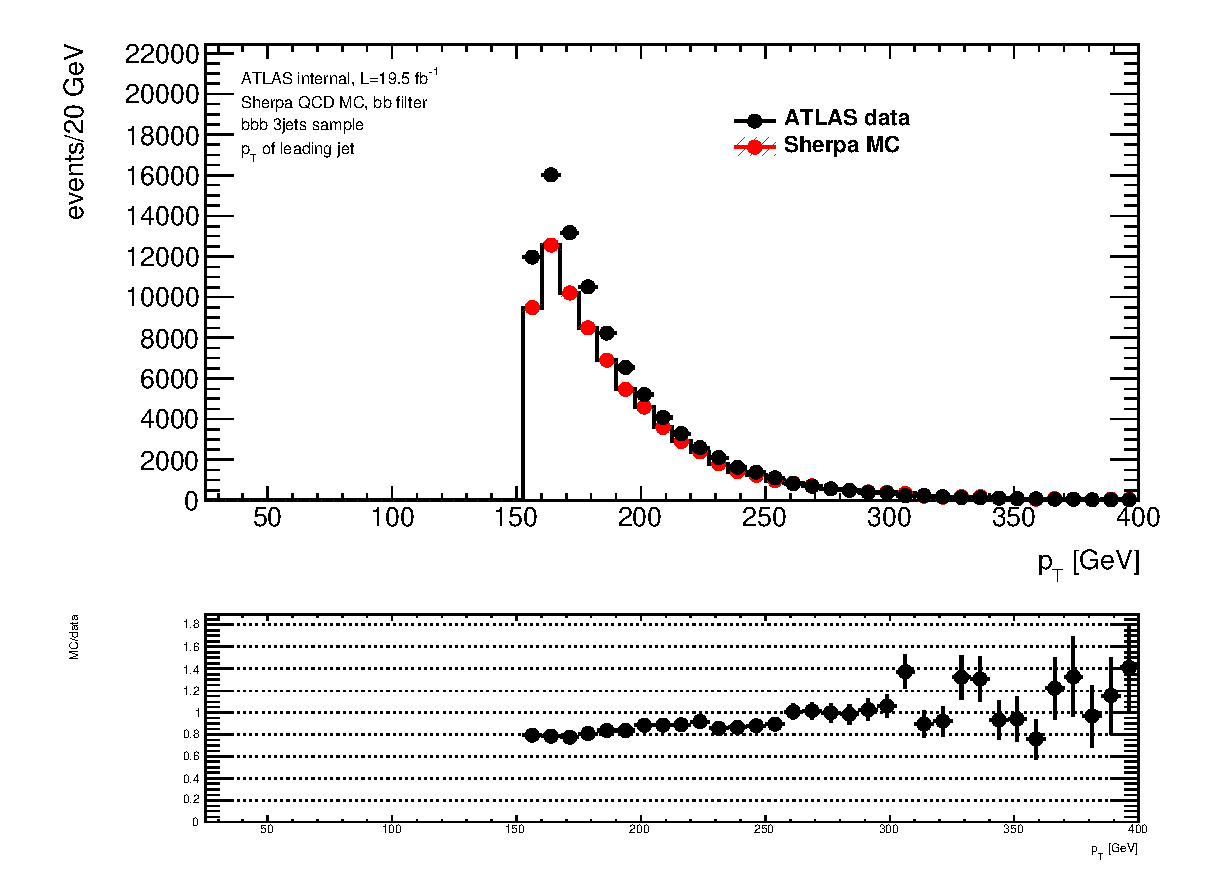
\includegraphics[width=\textwidth]{MonteCarlo/figures/pt0_bbb_3jets.eps}\end{subfigure}
  \begin{subfigure}[$bbb$ 4 jet category]{0.3\textwidth}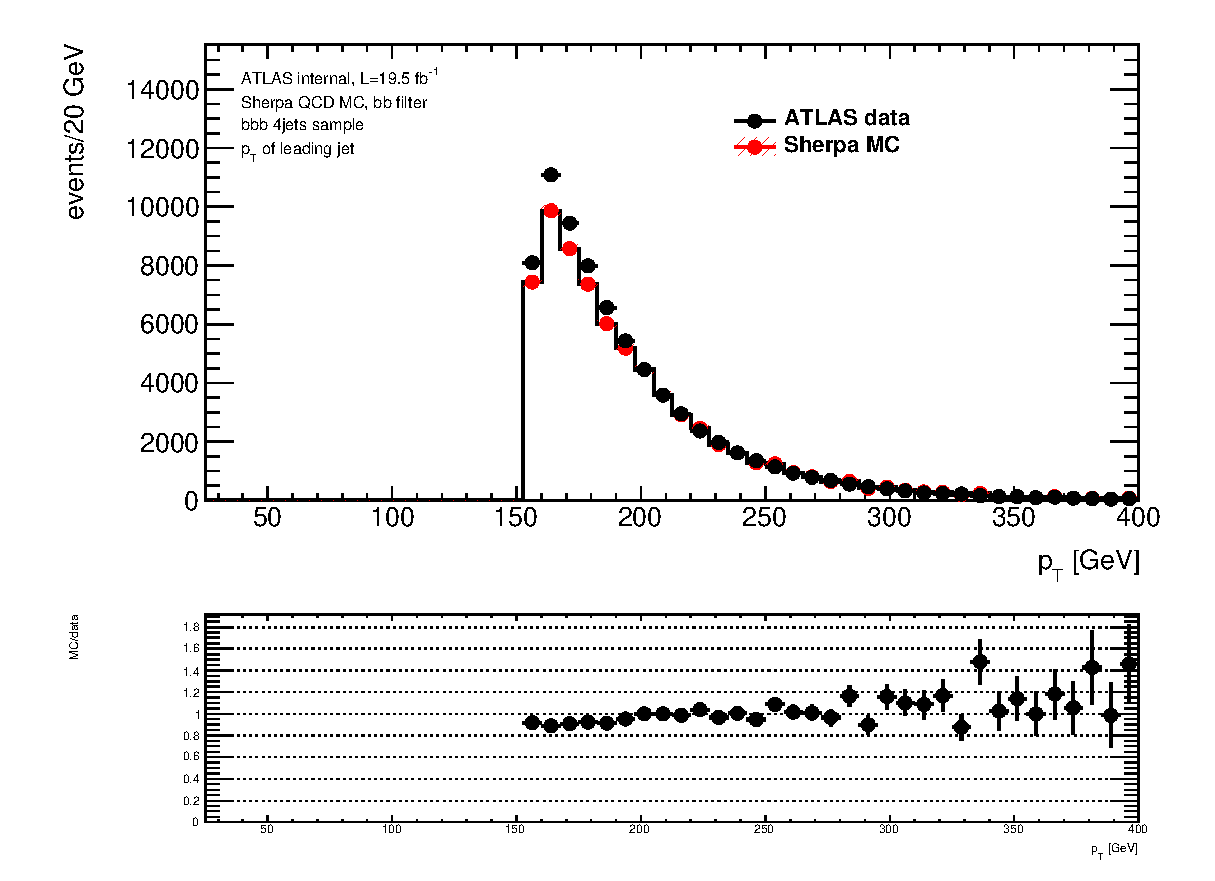
\includegraphics[width=\textwidth]{MonteCarlo/figures/pt0_bbb_4jets.eps}\end{subfigure}
  \begin{subfigure}[$bbb$ 5+ jet category]{0.3\textwidth}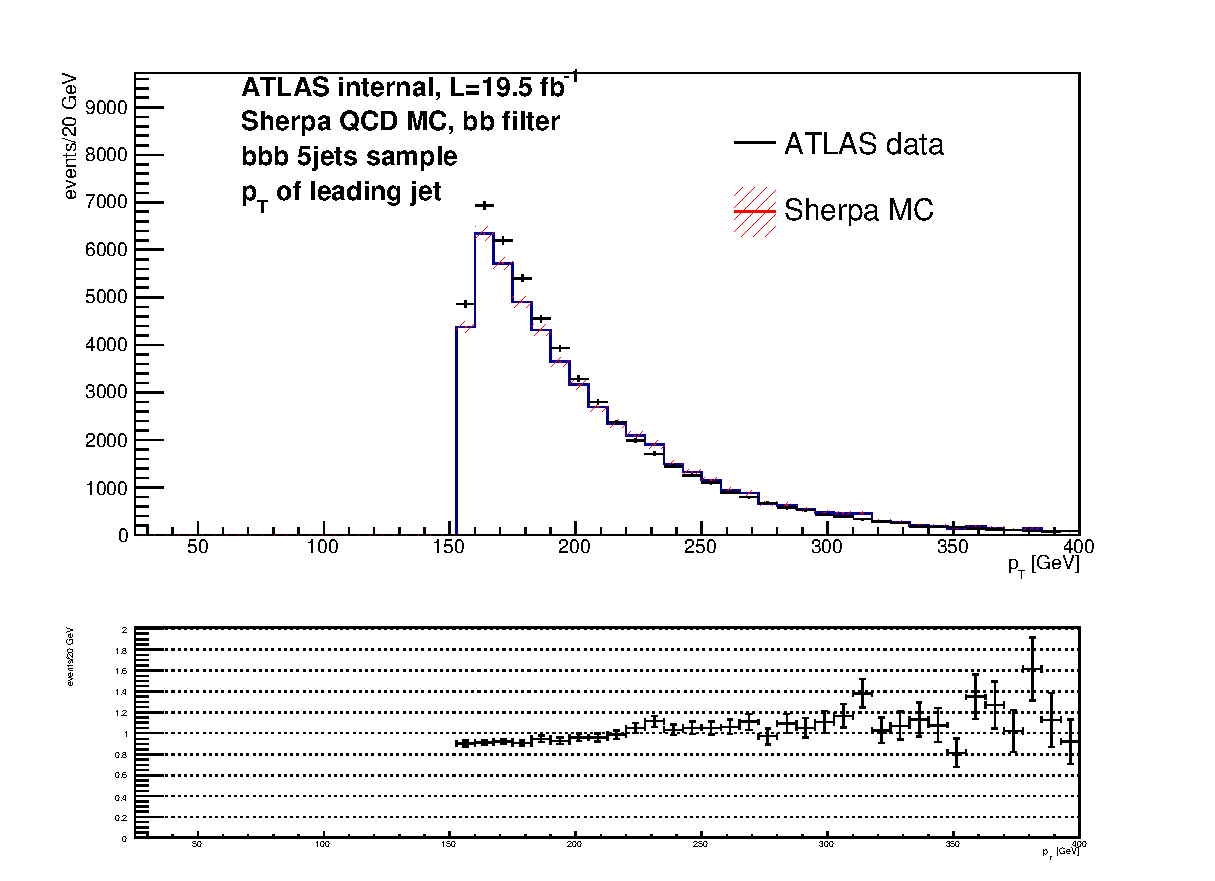
\includegraphics[width=\textwidth]{MonteCarlo/figures/pt0_bbb_5jets.eps}\end{subfigure}
  \begin{subfigure}[$bbloose$ 3 jet category]{0.3\textwidth}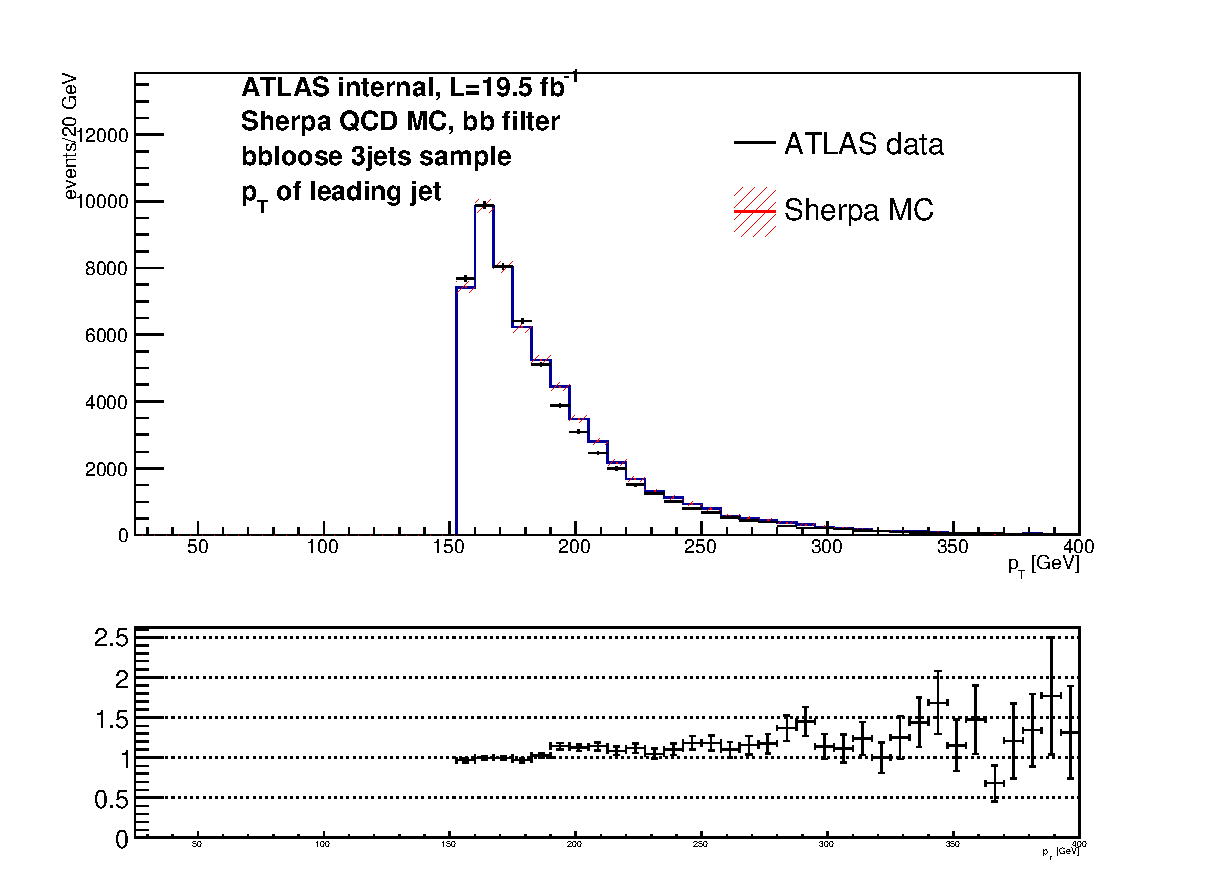
\includegraphics[width=\textwidth]{MonteCarlo/figures/pt0_bbloose_3jets.eps}\end{subfigure}
  \begin{subfigure}[$bbloose$ 4 jet category]{0.3\textwidth}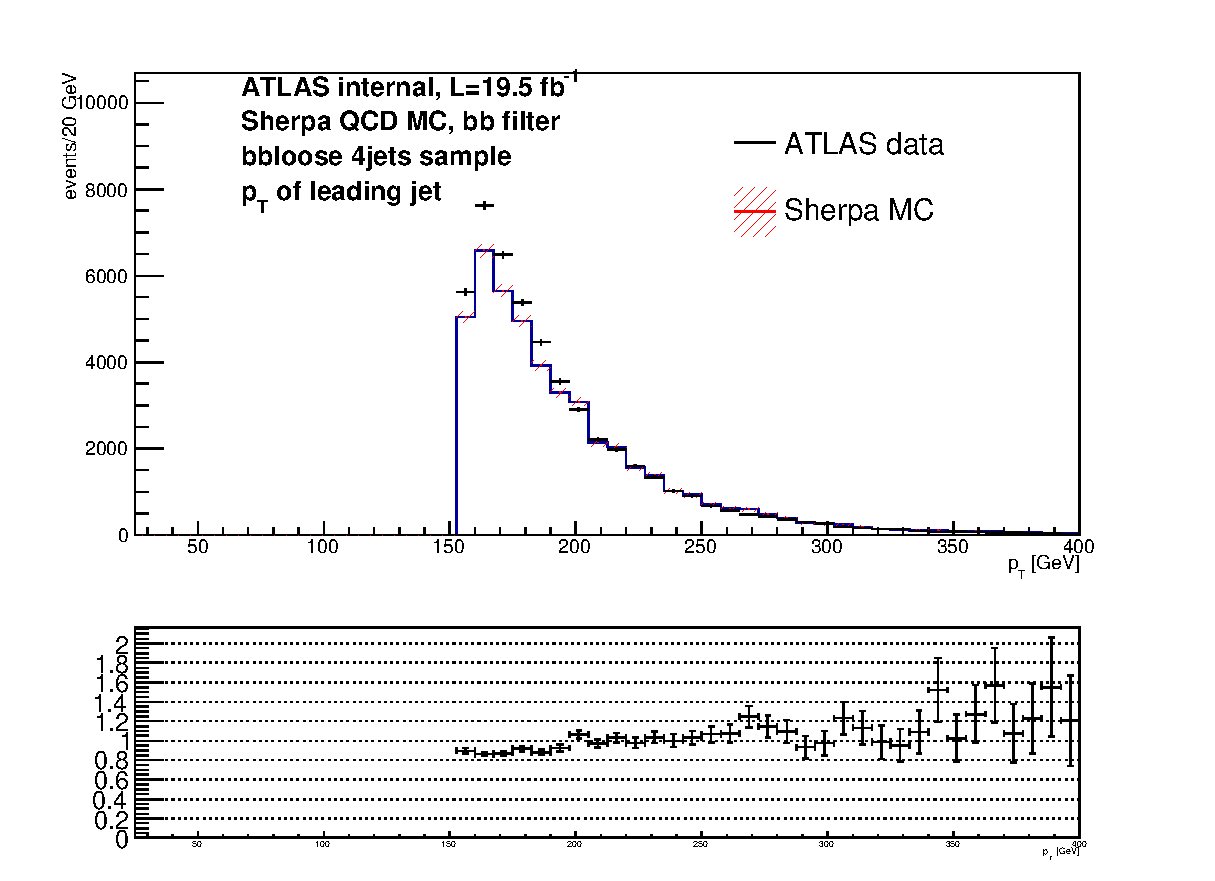
\includegraphics[width=\textwidth]{MonteCarlo/figures/pt0_bbloose_4jets.eps}\end{subfigure}
  \begin{subfigure}[$bbloose$ 5+ jet category]{0.3\textwidth}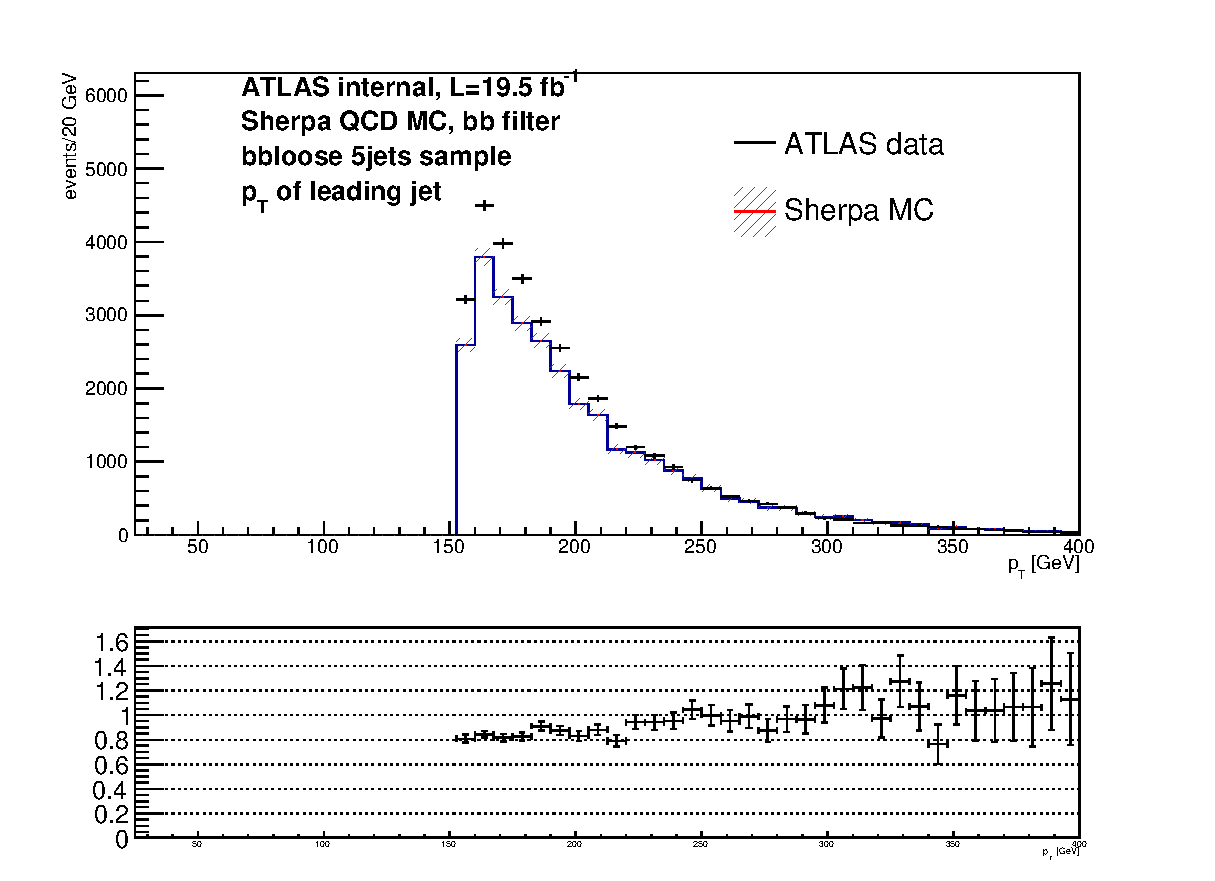
\includegraphics[width=\textwidth]{MonteCarlo/figures/pt0_bbloose_5jets.eps}\end{subfigure}
  \begin{subfigure}[$bbanti$ 3 jet category]{0.3\textwidth}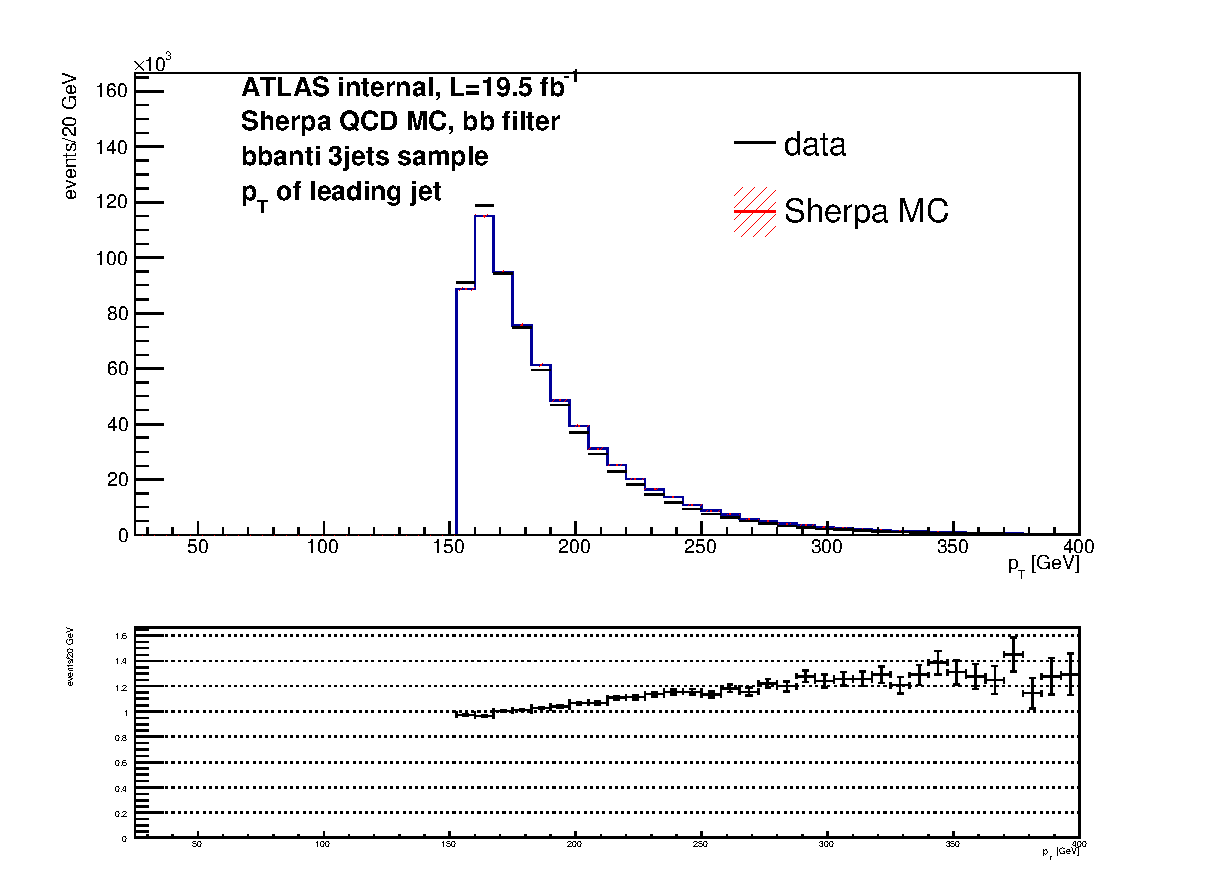
\includegraphics[width=\textwidth]{MonteCarlo/figures/pt0_bbanti_3jets.eps}\end{subfigure}
  \begin{subfigure}[$bbanti$ 4 jet category]{0.3\textwidth}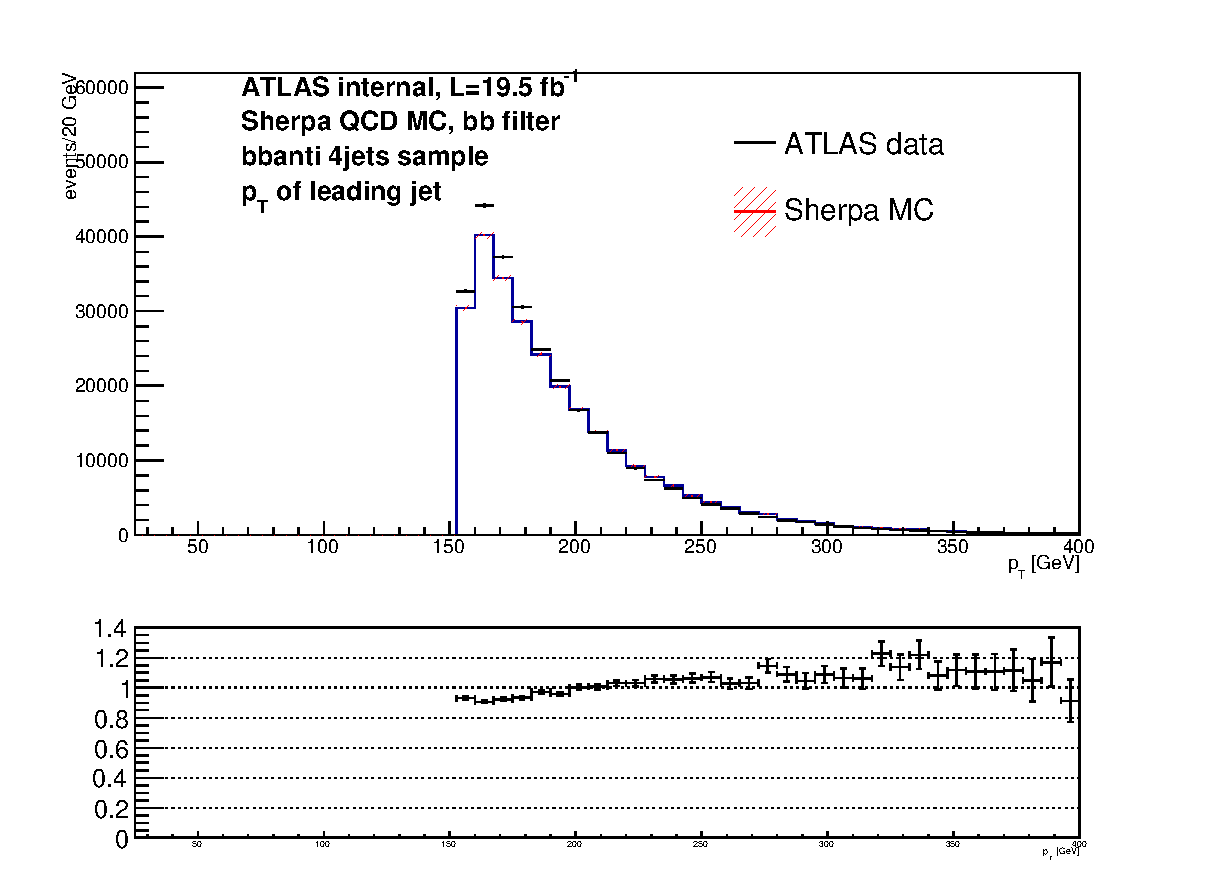
\includegraphics[width=\textwidth]{MonteCarlo/figures/pt0_bbanti_4jets.eps}\end{subfigure}
  \begin{subfigure}[$bbanti$ 5+ jet category]{0.3\textwidth}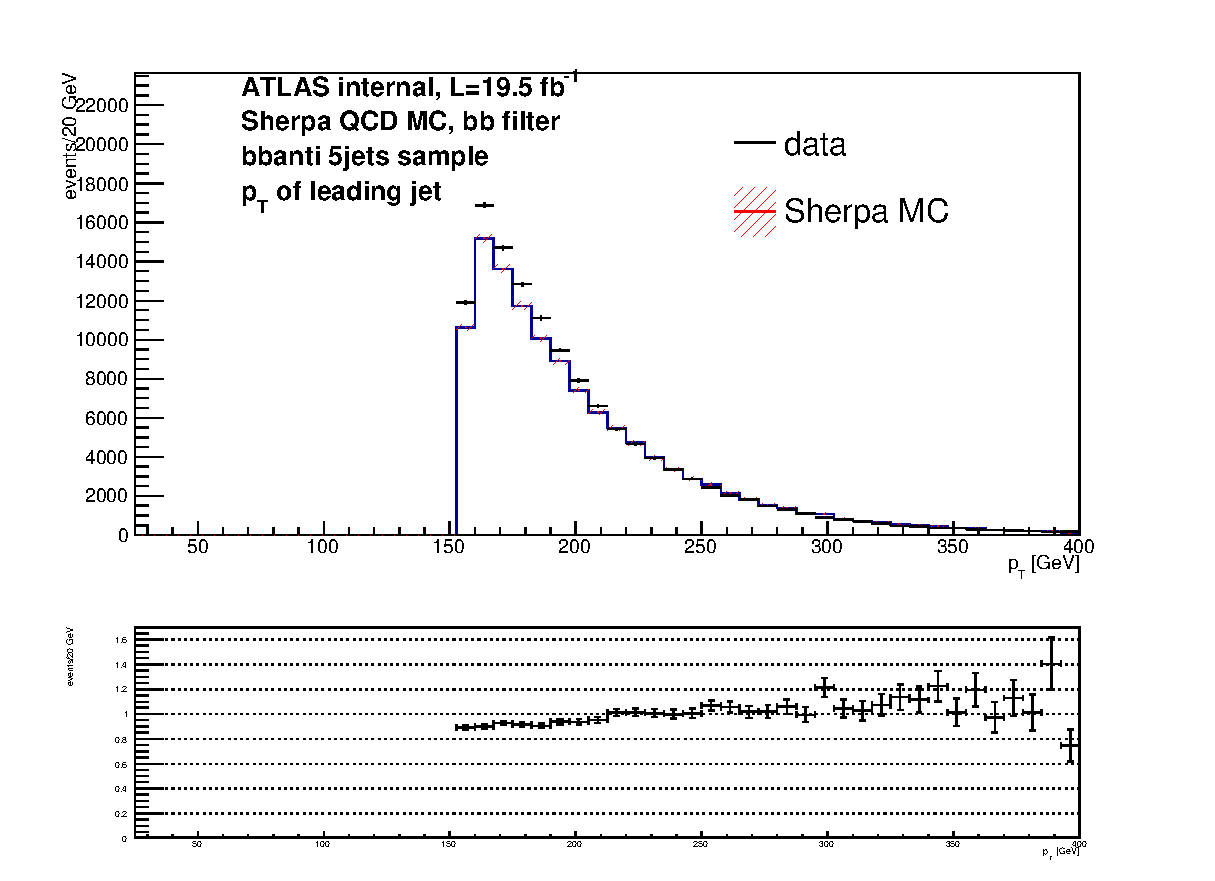
\includegraphics[width=\textwidth]{MonteCarlo/figures/pt0_bbanti_5jets.eps}\end{subfigure}
  \caption{The $p_T$ distributions for the leading jet, comparing bb QCD MC events to data.  The MC has been normalized
  to the same total number of events as the data (over the entire sample, not on a category-by-category basis)
  and the MC/data ratio is plotted in the lower subplots.  The errors on the MC are statistical only.
  \label{fig:bb_qcd_mc_pt0}}
    \end{center}
\end{figure}



\begin{figure}[phtb!]
  \begin{center}
  \begin{subfigure}[$bbb$ 3 jet category]{0.3\textwidth}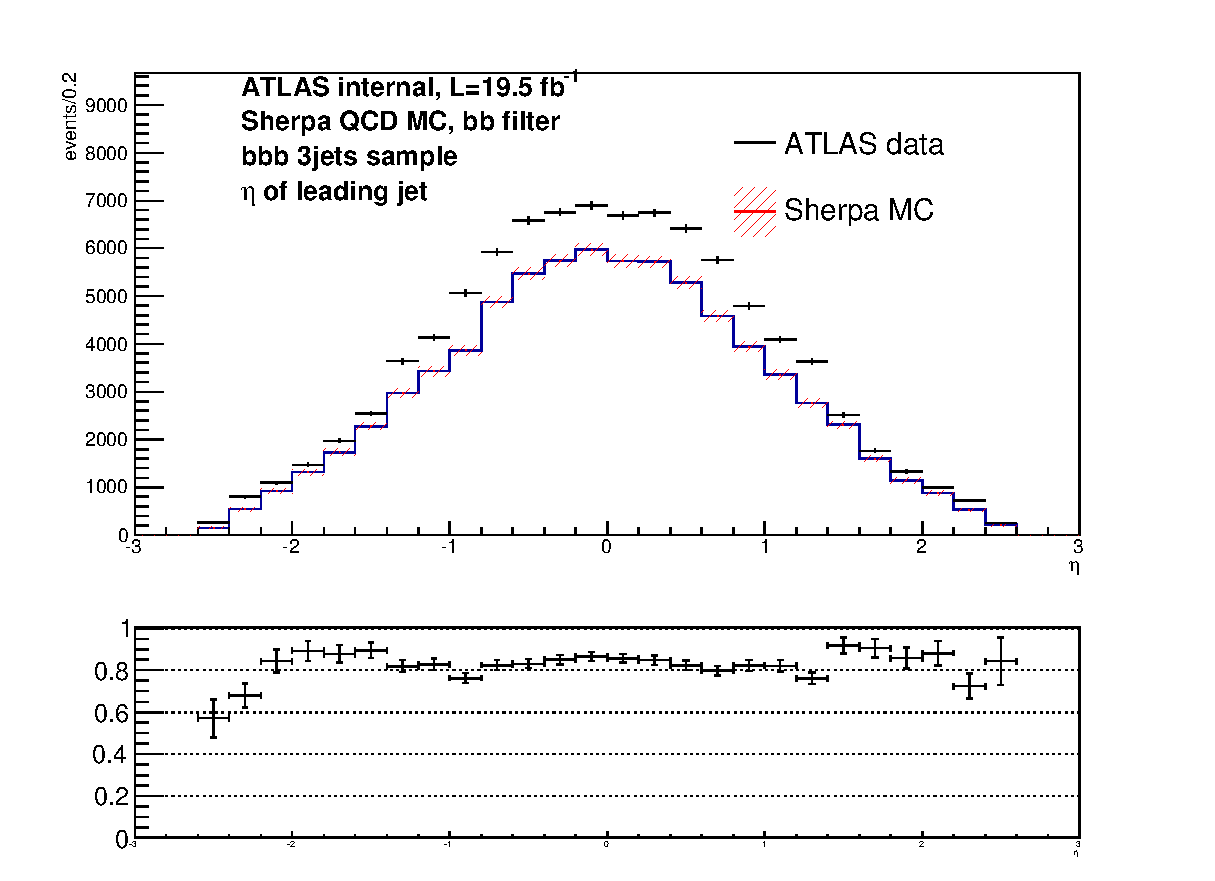
\includegraphics[width=\textwidth]{MonteCarlo/figures/eta0_bbb_3jets.eps}\end{subfigure}
  \begin{subfigure}[$bbb$ 4 jet category]{0.3\textwidth}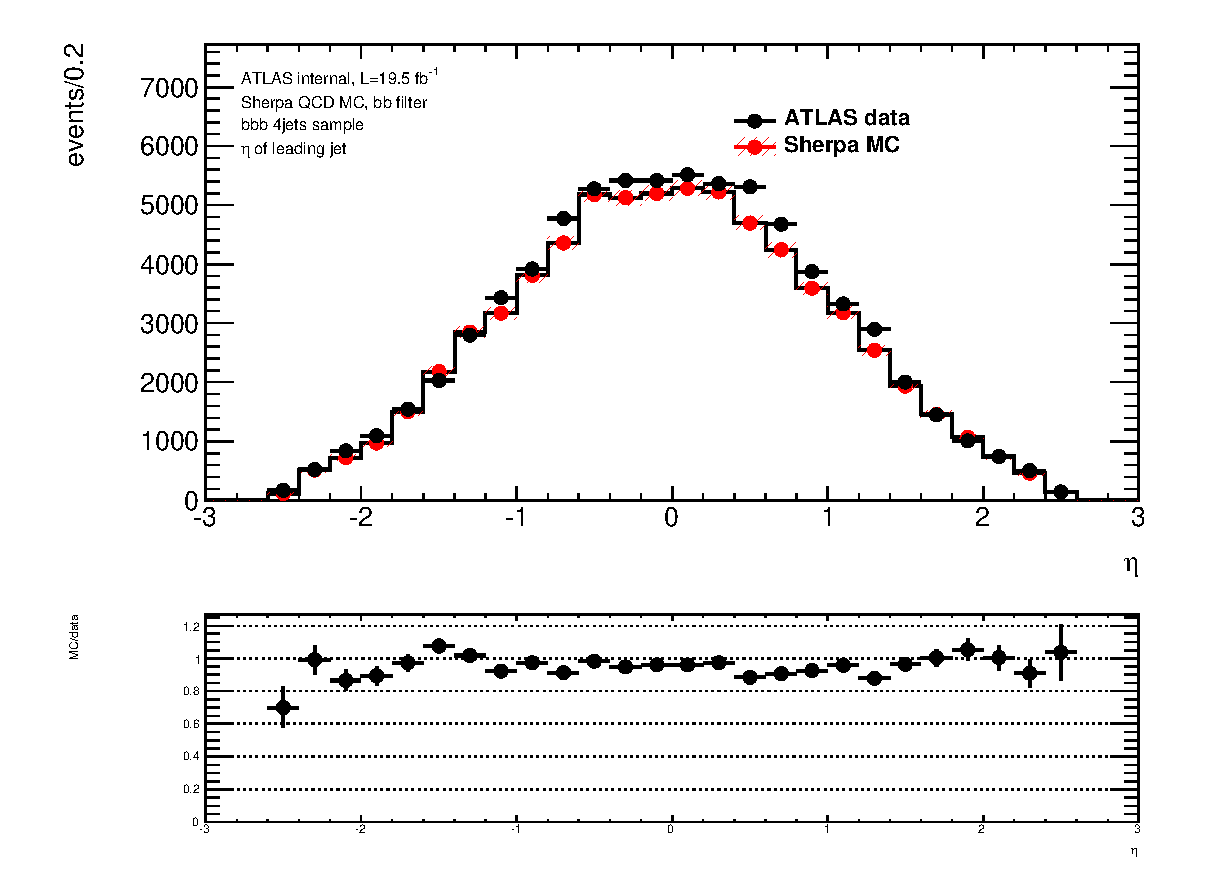
\includegraphics[width=\textwidth]{MonteCarlo/figures/eta0_bbb_4jets.eps}\end{subfigure}
  \begin{subfigure}[$bbb$ 5+ jet category]{0.3\textwidth}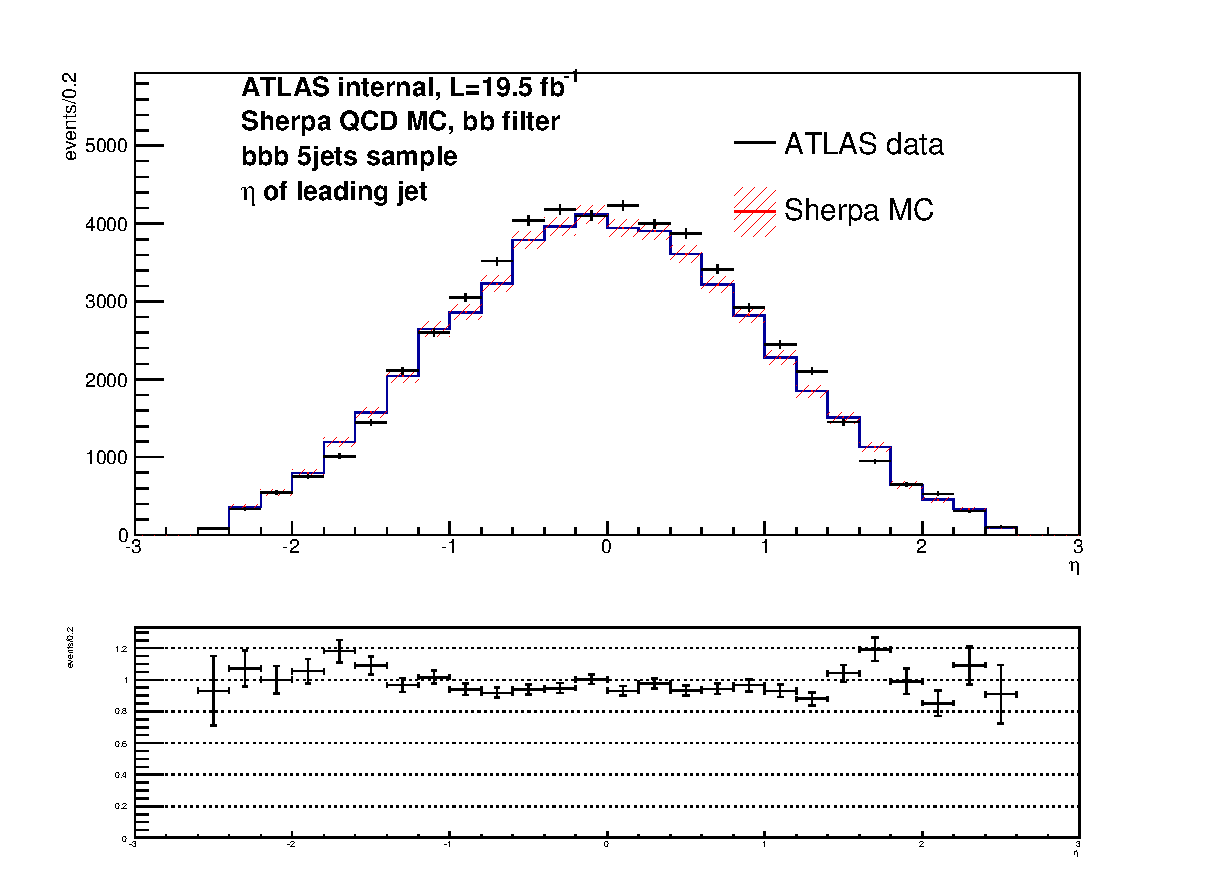
\includegraphics[width=\textwidth]{MonteCarlo/figures/eta0_bbb_5jets.eps}\end{subfigure}
  \begin{subfigure}[$bbloose$ 3 jet category]{0.3\textwidth}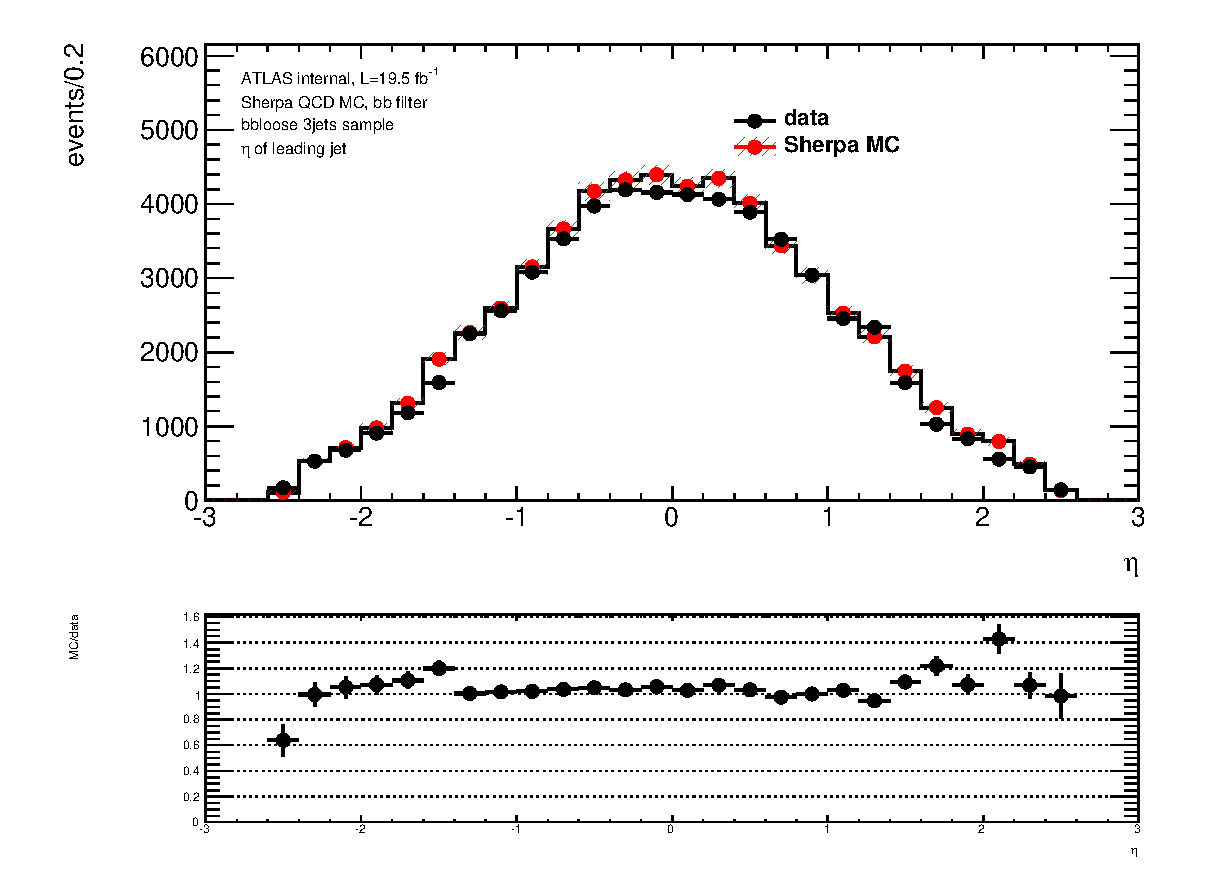
\includegraphics[width=\textwidth]{MonteCarlo/figures/eta0_bbloose_3jets.eps}\end{subfigure}
  \begin{subfigure}[$bbloose$ 4 jet category]{0.3\textwidth}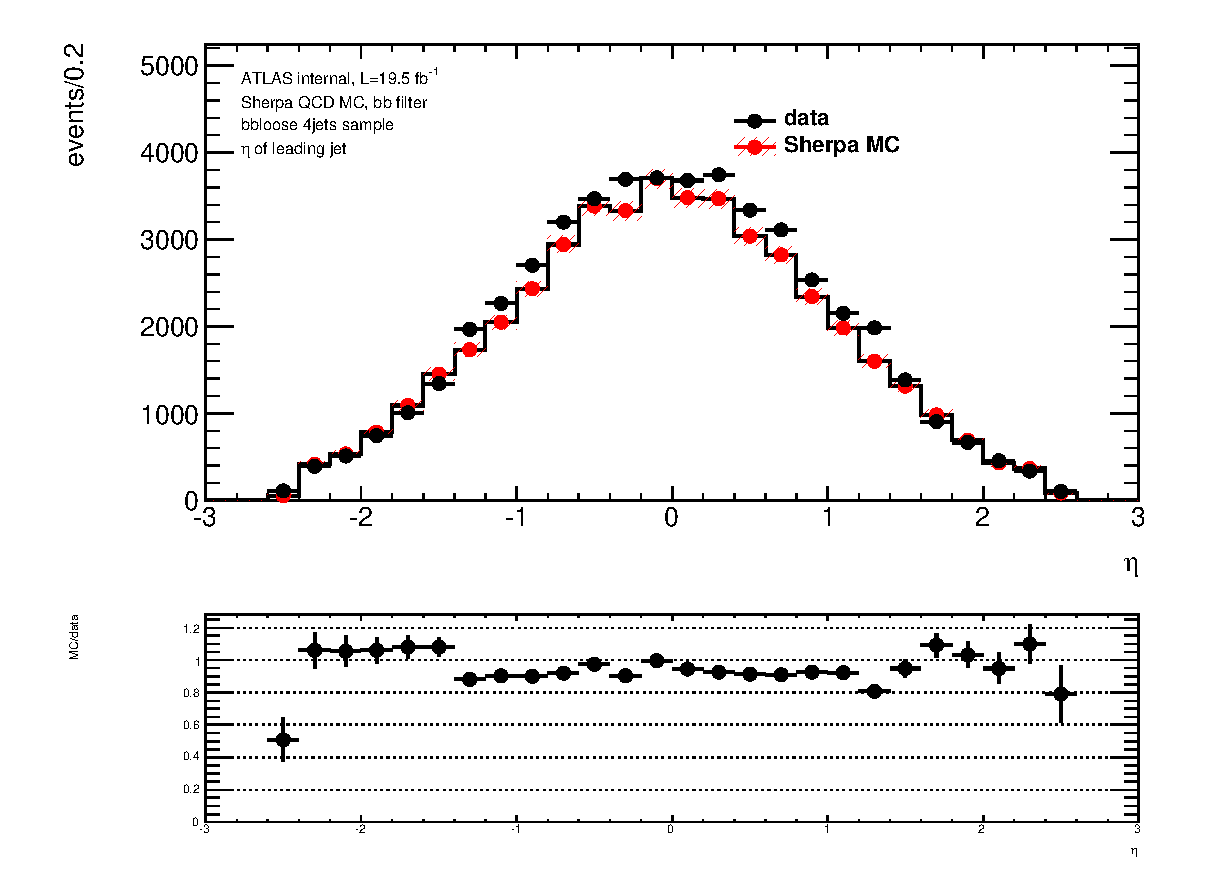
\includegraphics[width=\textwidth]{MonteCarlo/figures/eta0_bbloose_4jets.eps}\end{subfigure}
  \begin{subfigure}[$bbloose$ 5+ jet category]{0.3\textwidth}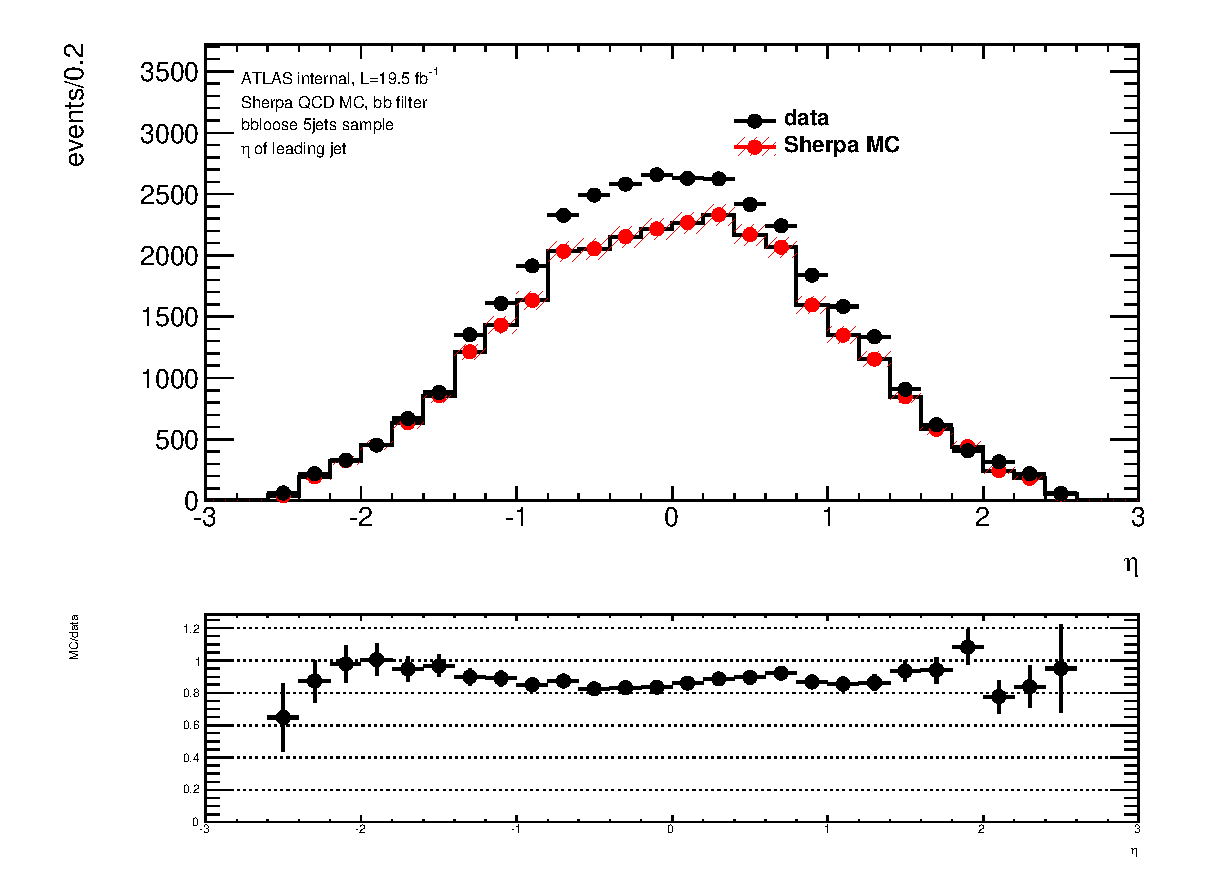
\includegraphics[width=\textwidth]{MonteCarlo/figures/eta0_bbloose_5jets.eps}\end{subfigure}
  \begin{subfigure}[$bbanti$ 3 jet category]{0.3\textwidth}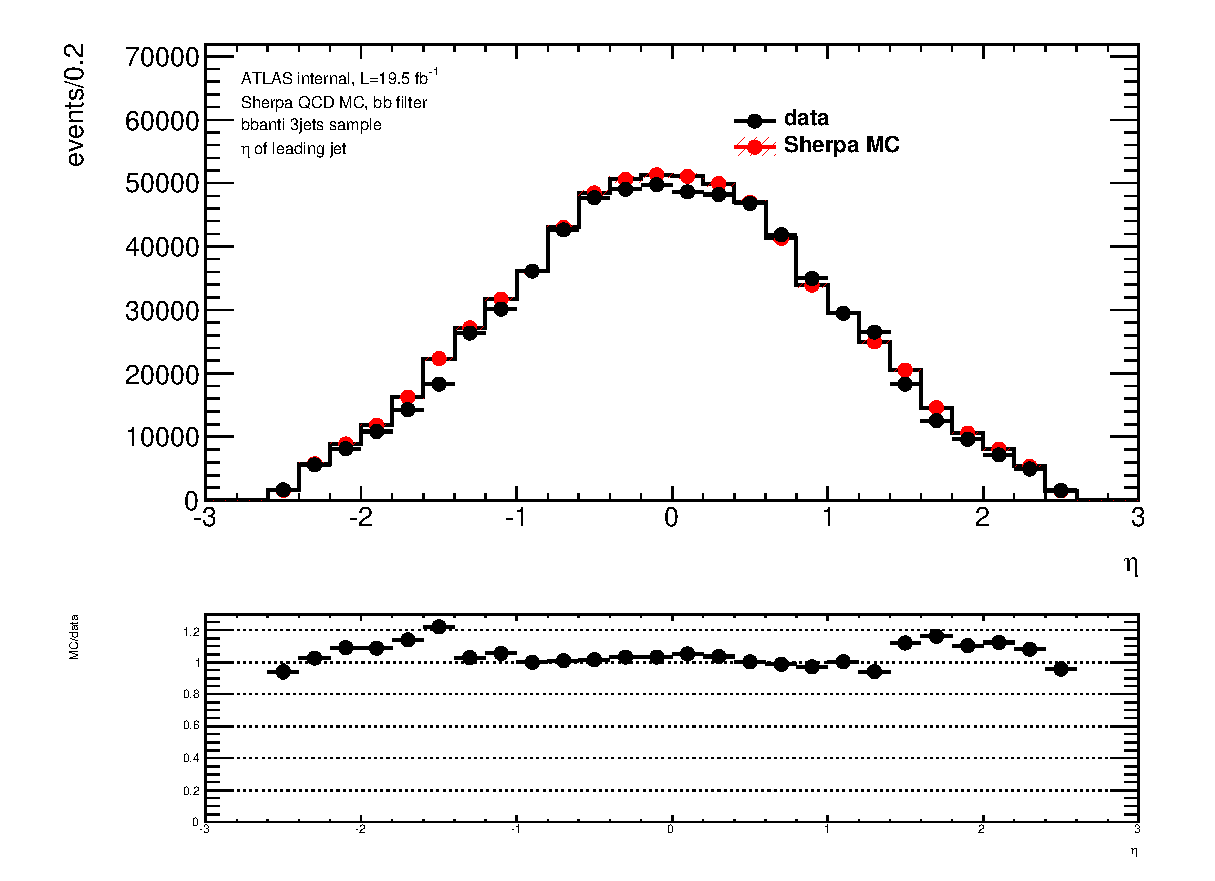
\includegraphics[width=\textwidth]{MonteCarlo/figures/eta0_bbanti_3jets.eps}\end{subfigure}
  \begin{subfigure}[$bbanti$ 4 jet category]{0.3\textwidth}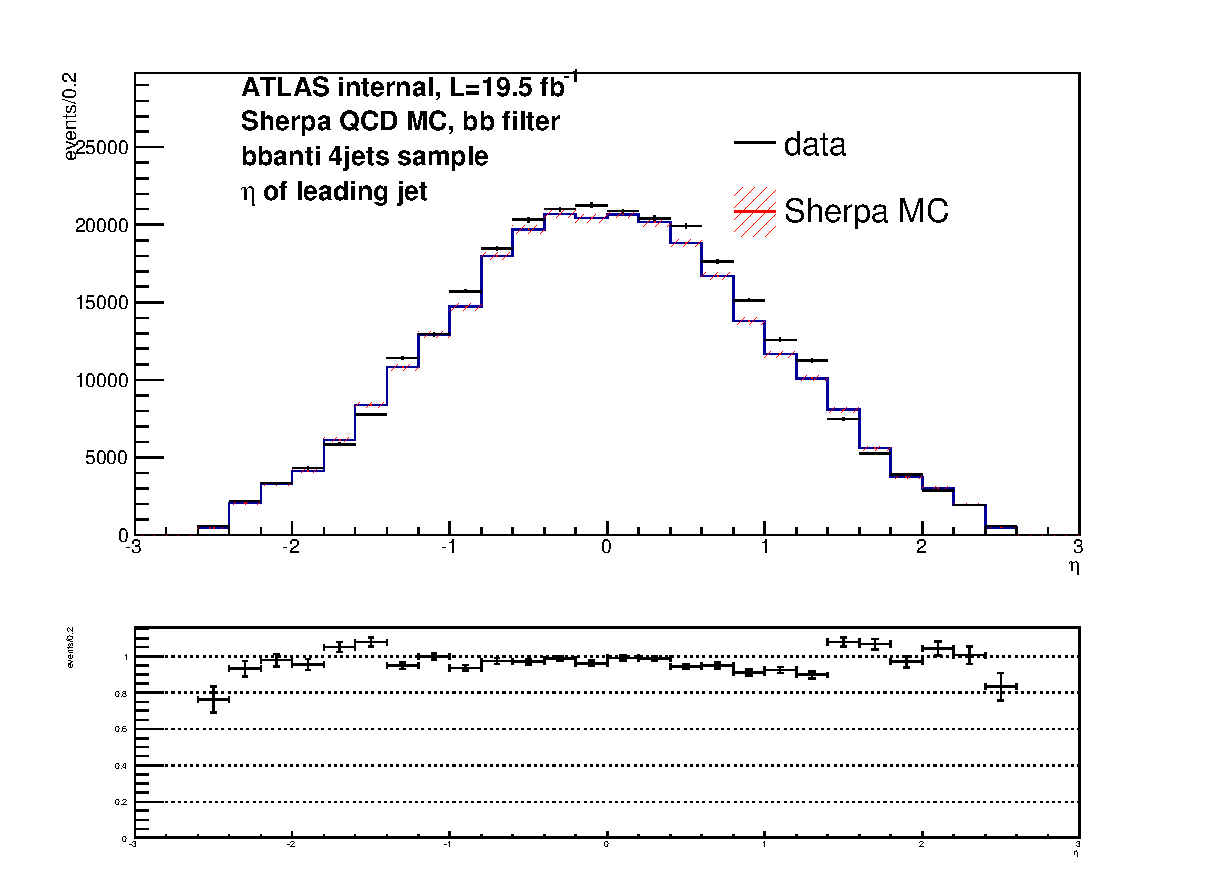
\includegraphics[width=\textwidth]{MonteCarlo/figures/eta0_bbanti_4jets.eps}\end{subfigure}
  \begin{subfigure}[$bbanti$ 5+ jet category]{0.3\textwidth}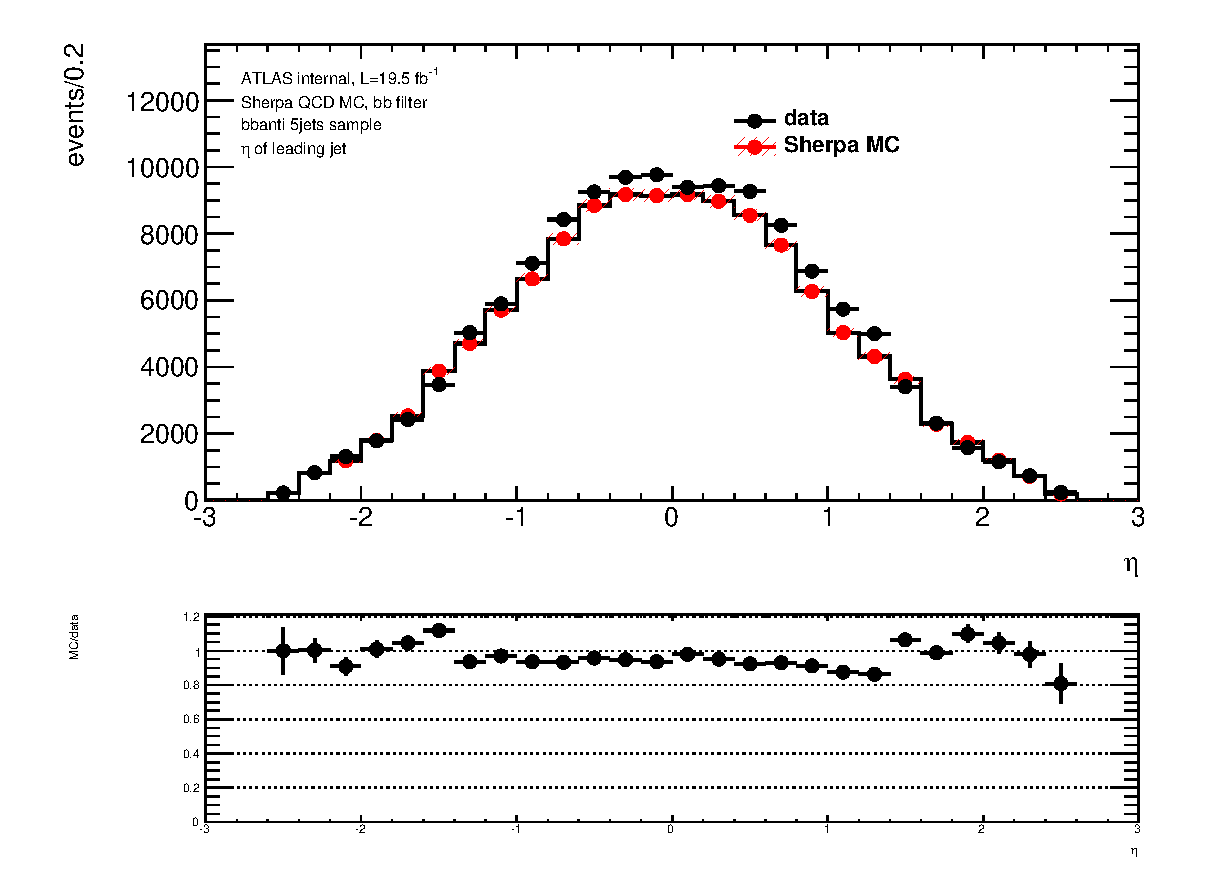
\includegraphics[width=\textwidth]{MonteCarlo/figures/eta0_bbanti_5jets.eps}\end{subfigure}
  \caption{The $\eta$ distributions for the leading jet, comparing bb QCD MC events to data.  The MC has been normalized
  to the same total number of events as the data (over the entire sample, not on a category-by-category basis)
  and the MC/data ratio is plotted in the lower subplots.  The errors on the MC are statistical only.
  \label{fig:bb_qcd_mc_eta0}}
    \end{center}
\end{figure}



\begin{figure}[phtb!]
  \begin{center}
  \begin{subfigure}[$bbb$ 3 jet category]{0.3\textwidth}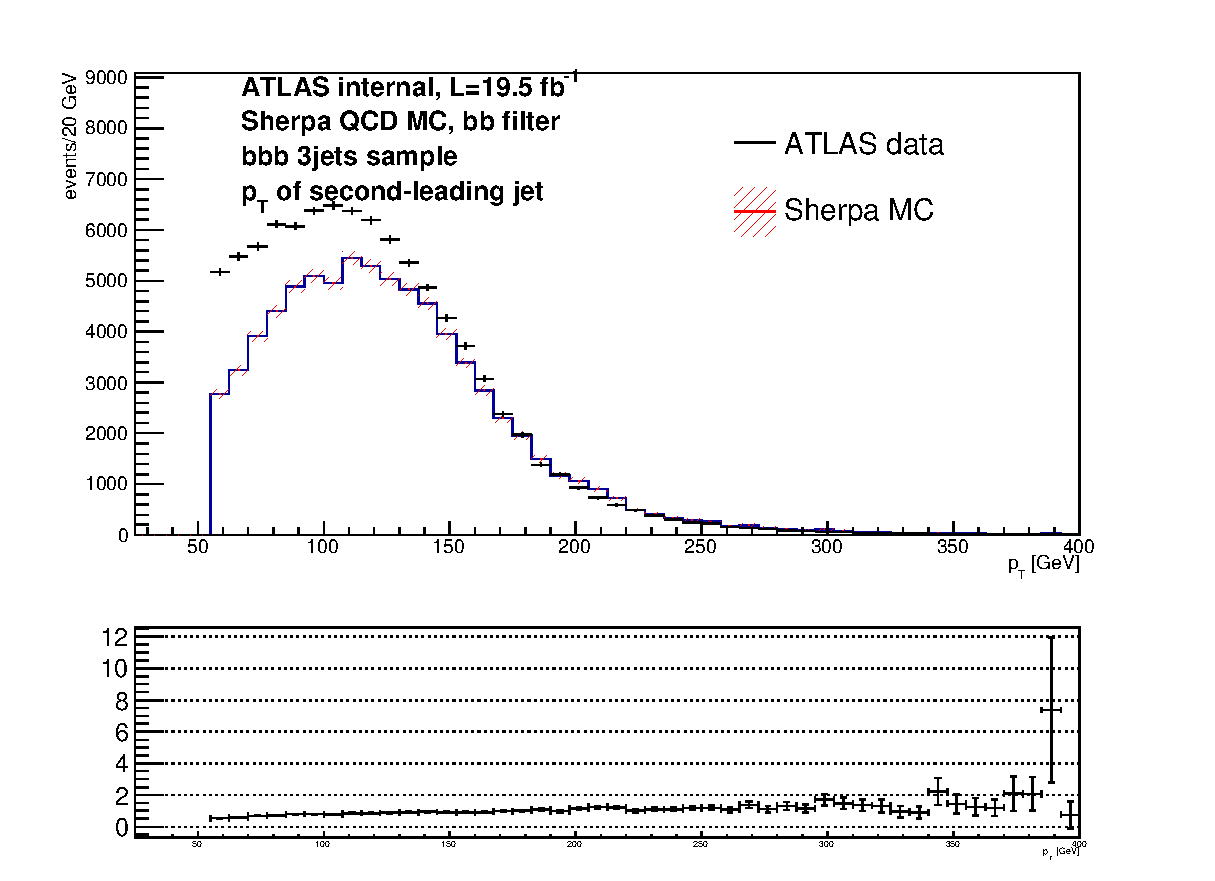
\includegraphics[width=\textwidth]{MonteCarlo/figures/pt1_bbb_3jets.eps}\end{subfigure}
  \begin{subfigure}[$bbb$ 4 jet category]{0.3\textwidth}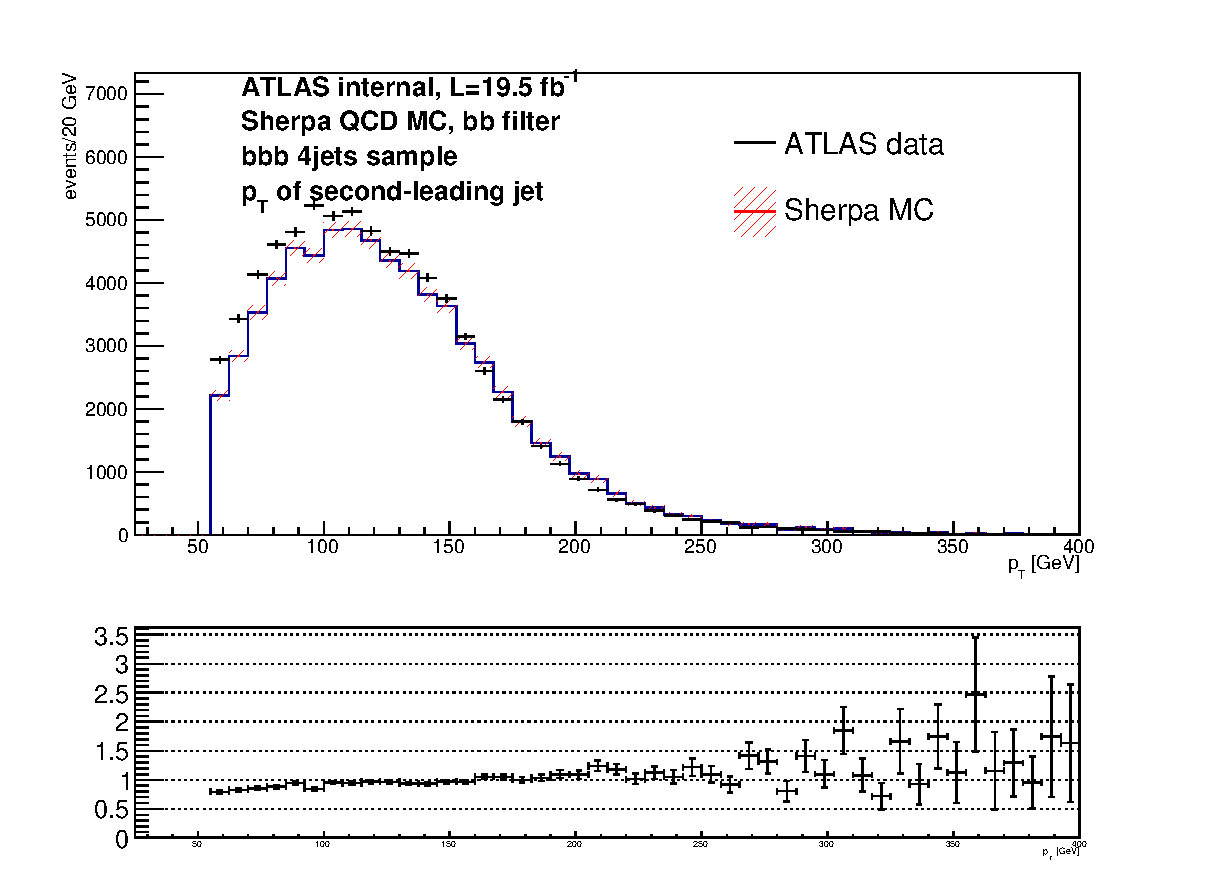
\includegraphics[width=\textwidth]{MonteCarlo/figures/pt1_bbb_4jets.eps}\end{subfigure}
  \begin{subfigure}[$bbb$ 5+ jet category]{0.3\textwidth}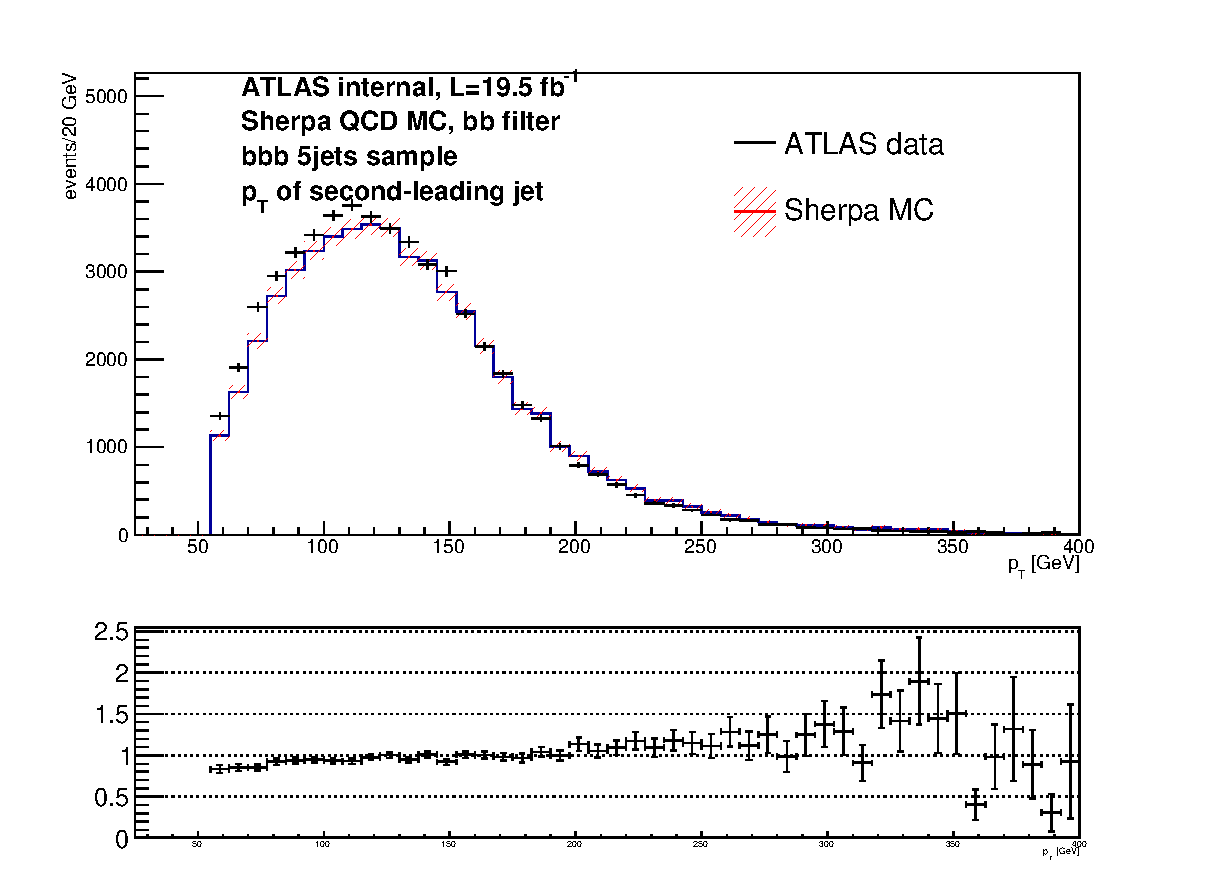
\includegraphics[width=\textwidth]{MonteCarlo/figures/pt1_bbb_5jets.eps}\end{subfigure}
  \begin{subfigure}[$bbloose$ 3 jet category]{0.3\textwidth}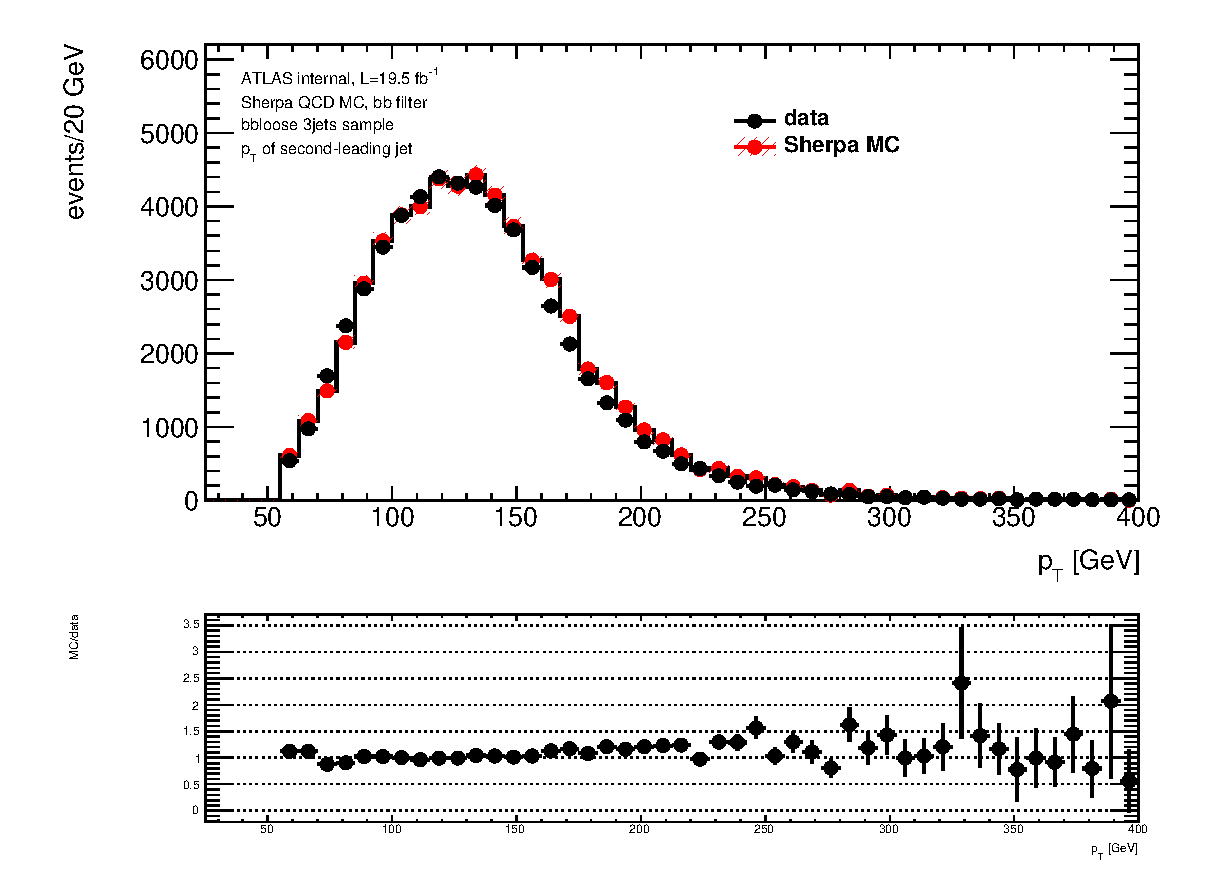
\includegraphics[width=\textwidth]{MonteCarlo/figures/pt1_bbloose_3jets.eps}\end{subfigure}
  \begin{subfigure}[$bbloose$ 4 jet category]{0.3\textwidth}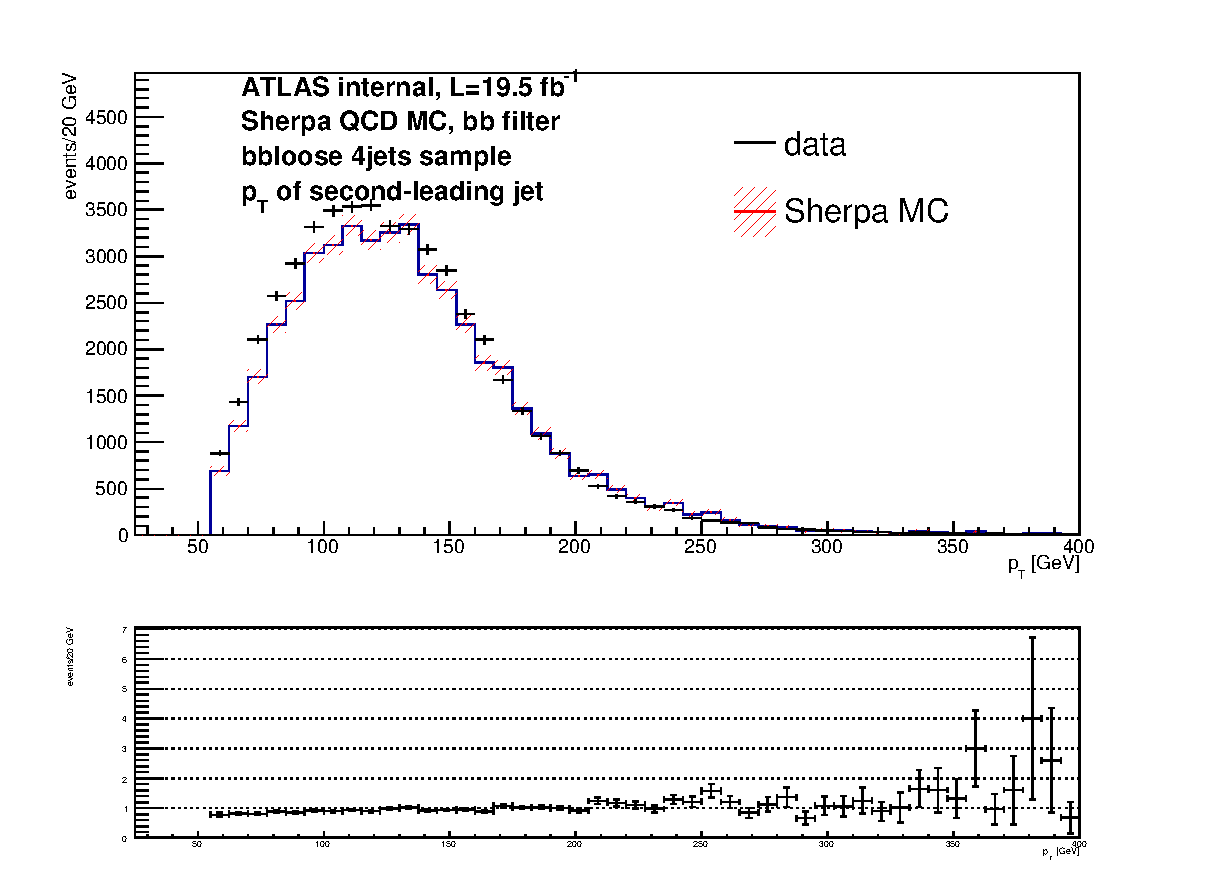
\includegraphics[width=\textwidth]{MonteCarlo/figures/pt1_bbloose_4jets.eps}\end{subfigure}
  \begin{subfigure}[$bbloose$ 5+ jet category]{0.3\textwidth}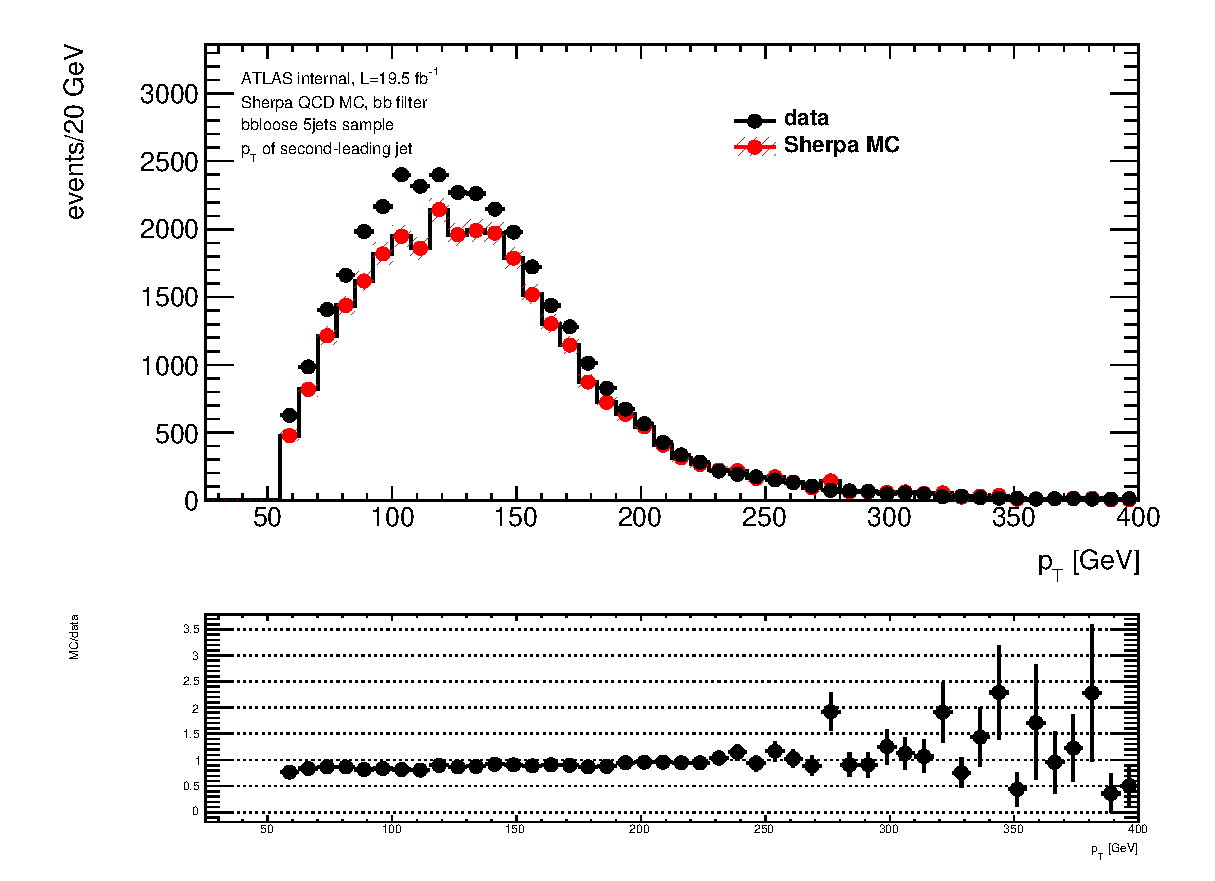
\includegraphics[width=\textwidth]{MonteCarlo/figures/pt1_bbloose_5jets.eps}\end{subfigure}
  \begin{subfigure}[$bbanti$ 3 jet category]{0.3\textwidth}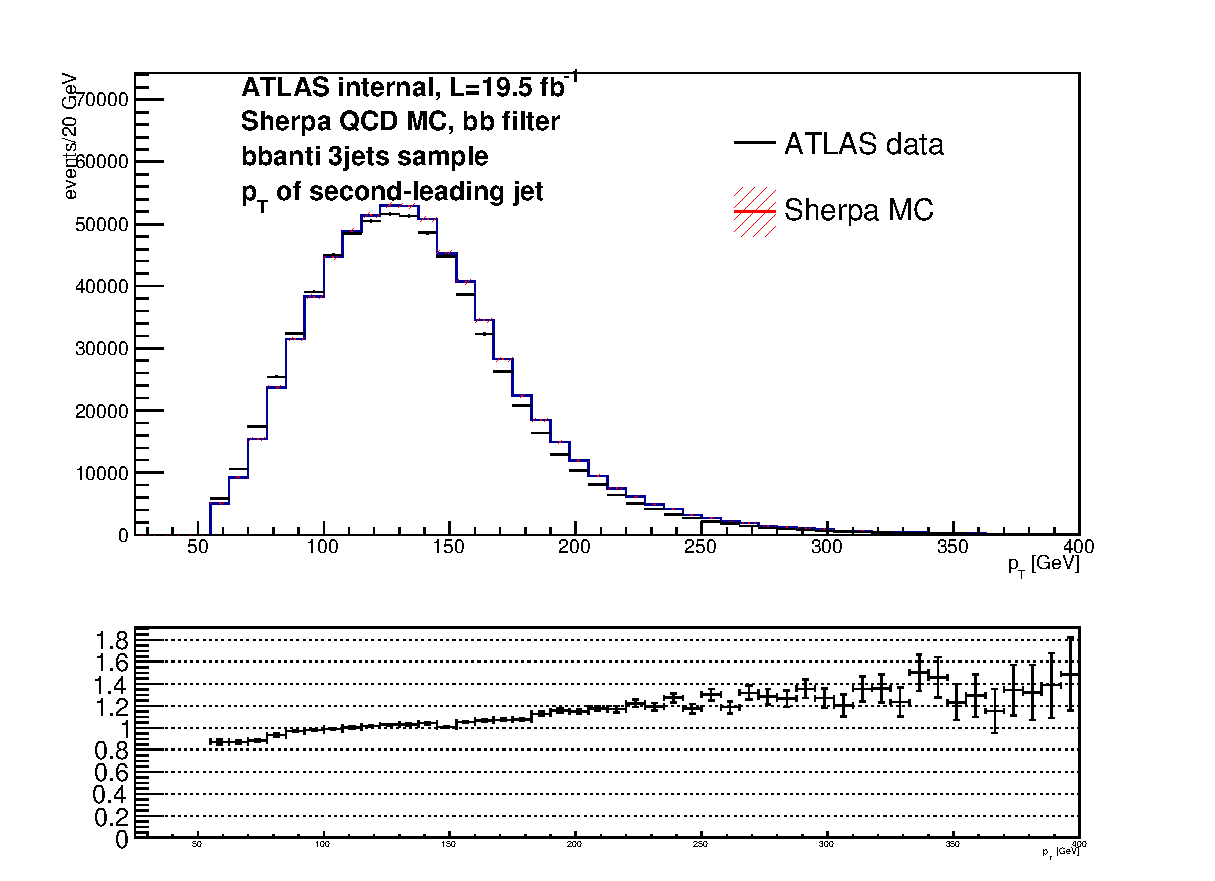
\includegraphics[width=\textwidth]{MonteCarlo/figures/pt1_bbanti_3jets.eps}\end{subfigure}
  \begin{subfigure}[$bbanti$ 4 jet category]{0.3\textwidth}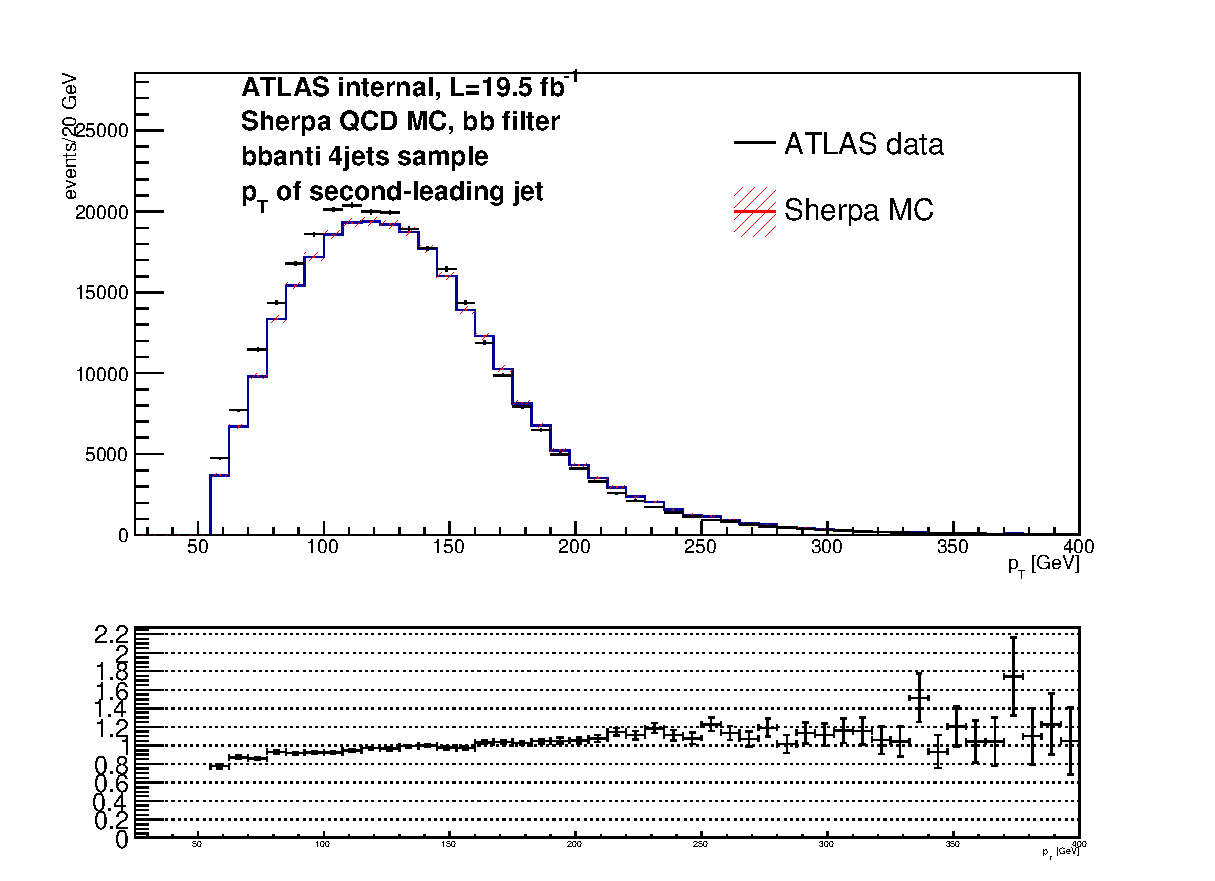
\includegraphics[width=\textwidth]{MonteCarlo/figures/pt1_bbanti_4jets.eps}\end{subfigure}
  \begin{subfigure}[$bbanti$ 5+ jet category]{0.3\textwidth}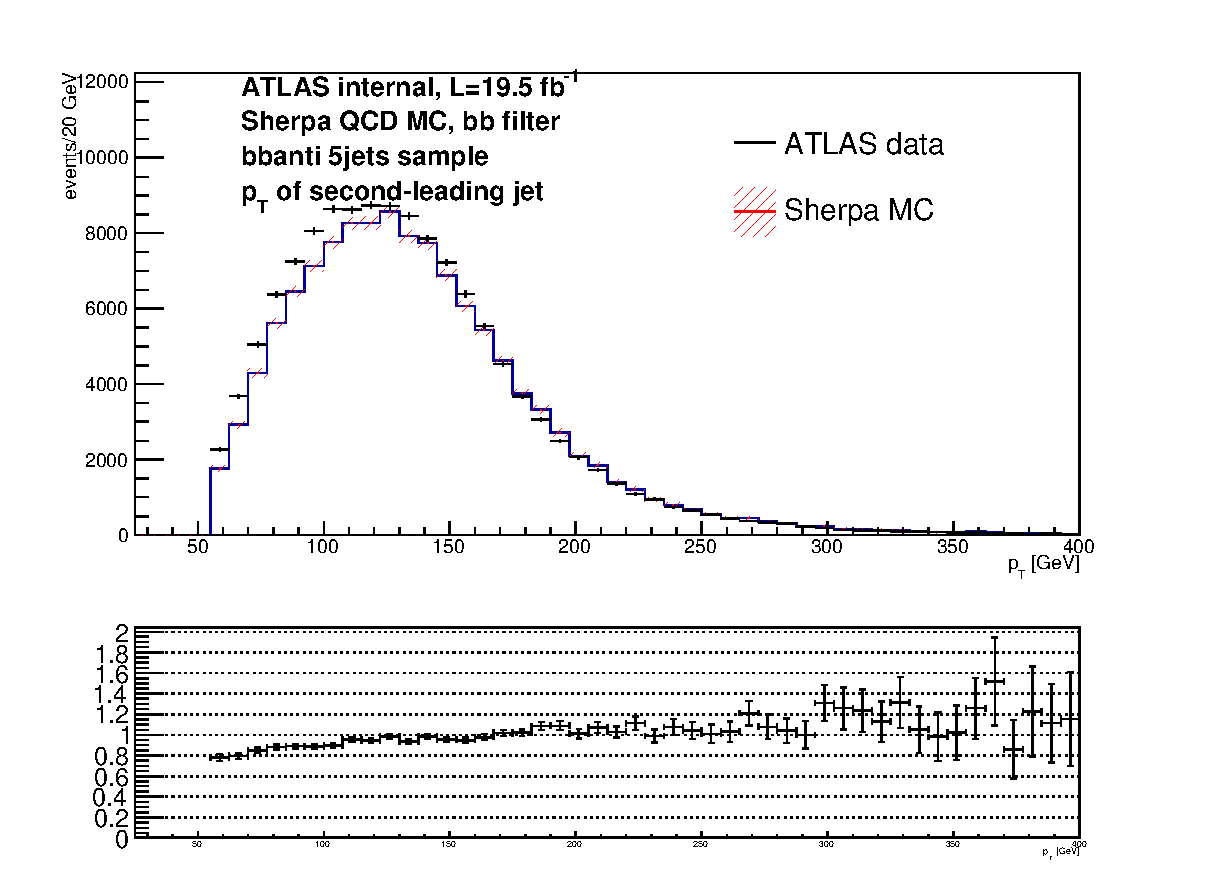
\includegraphics[width=\textwidth]{MonteCarlo/figures/pt1_bbanti_5jets.eps}\end{subfigure}
  \caption{The $p_T$ distributions for the second-leading jet, comparing bb QCD MC events to data.  The MC has been normalized
  to the same total number of events as the data (over the entire sample, not on a category-by-category basis)
  and the MC/data ratio is plotted in the lower subplots.  The errors on the MC are statistical only.
  \label{fig:bb_qcd_mc_pt1}}
    \end{center}
\end{figure}

\begin{figure}[phtb!]
  \begin{center}
  \begin{subfigure}[$bbb$ 3 jet category]{0.3\textwidth}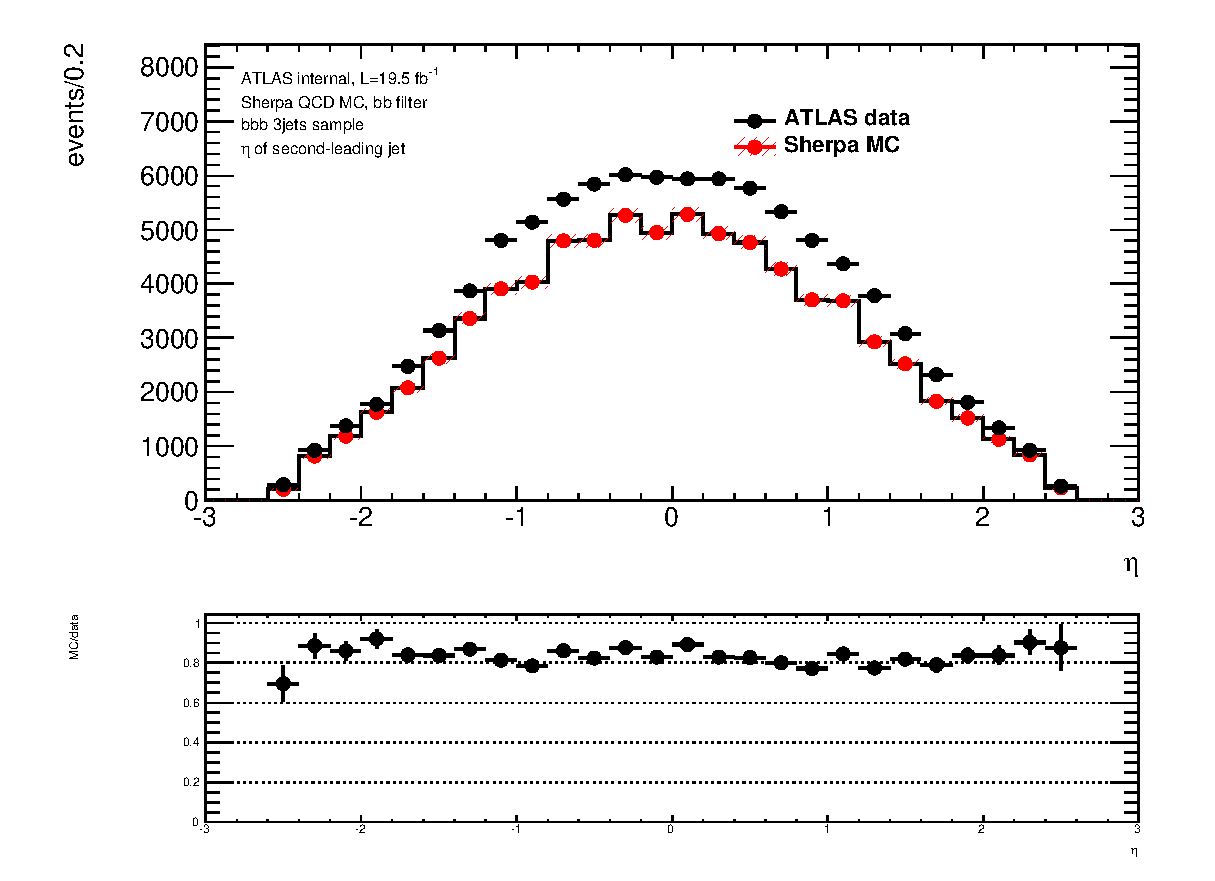
\includegraphics[width=\textwidth]{MonteCarlo/figures/eta1_bbb_3jets.eps}\end{subfigure}
  \begin{subfigure}[$bbb$ 4 jet category]{0.3\textwidth}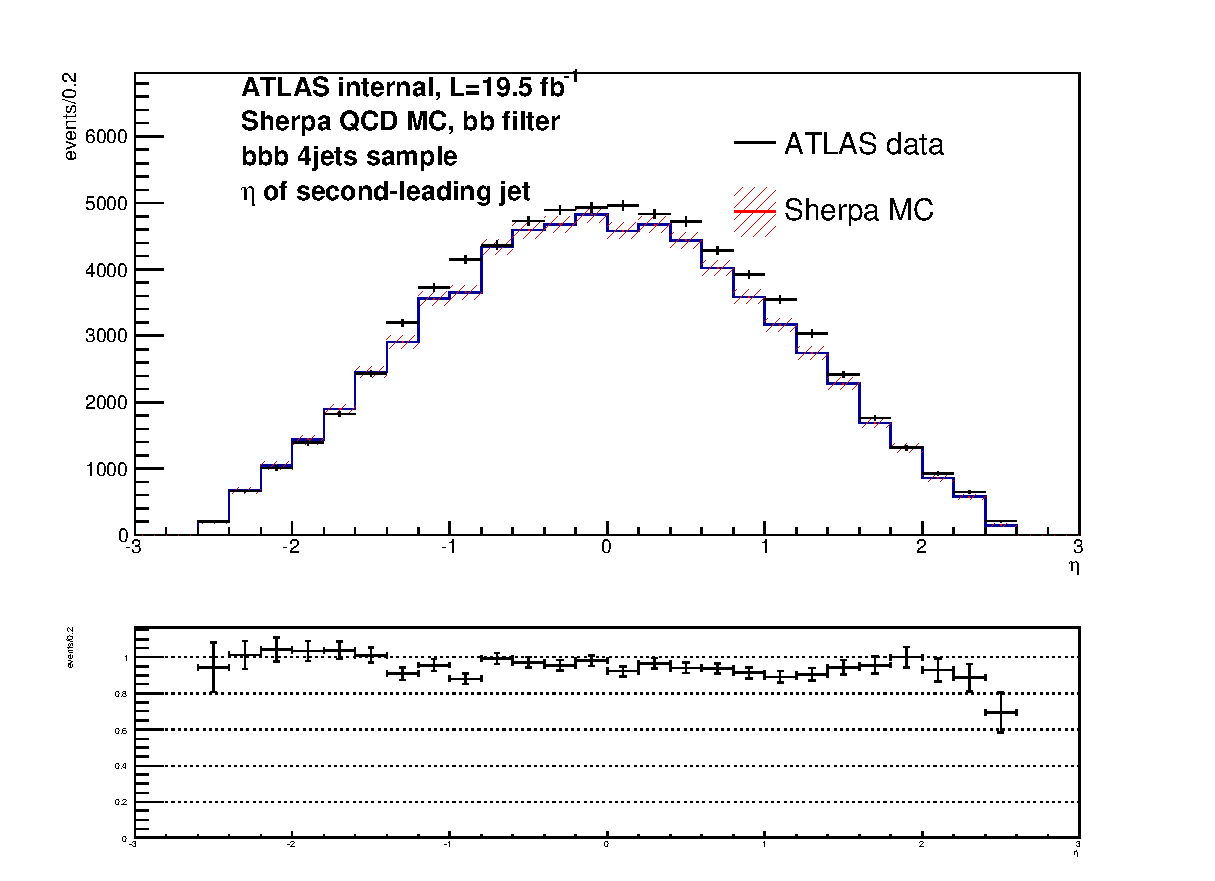
\includegraphics[width=\textwidth]{MonteCarlo/figures/eta1_bbb_4jets.eps}\end{subfigure}
  \begin{subfigure}[$bbb$ 5+ jet category]{0.3\textwidth}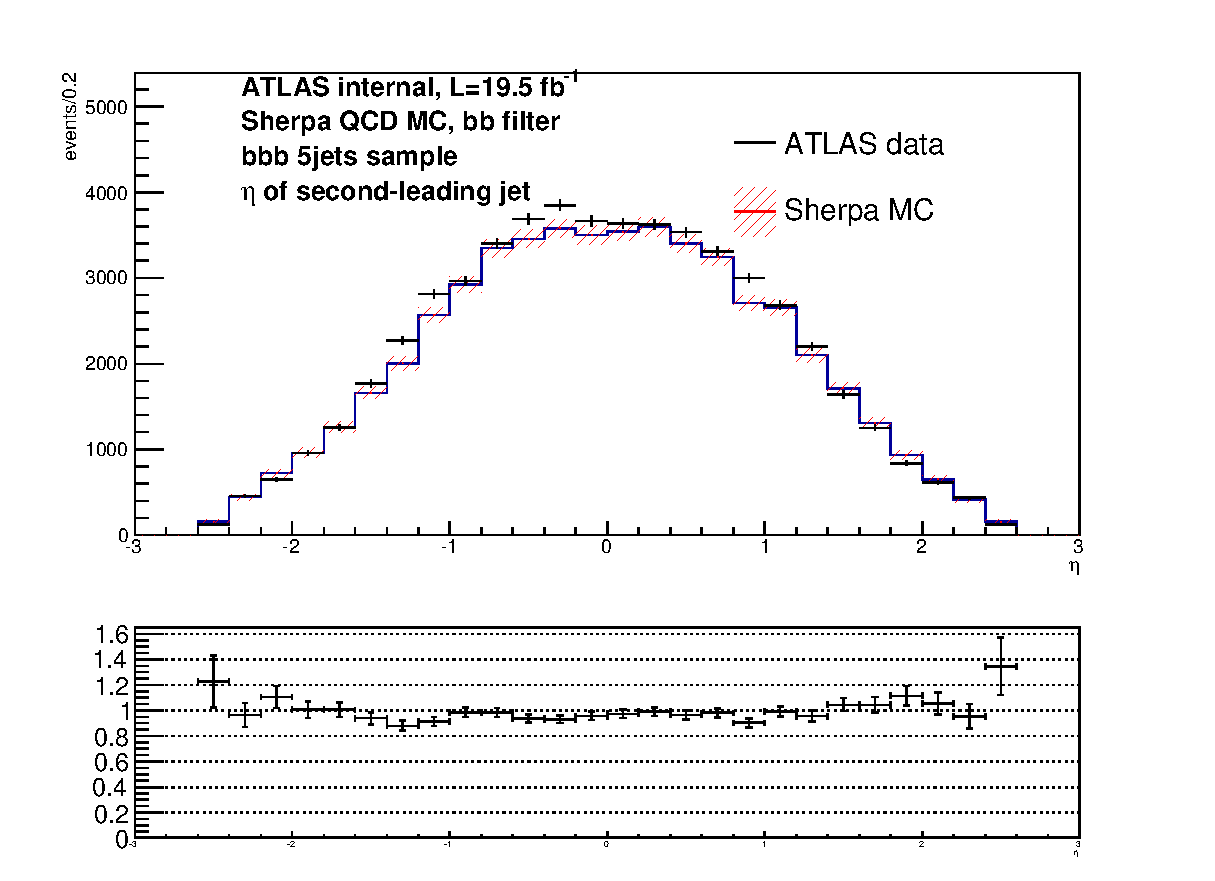
\includegraphics[width=\textwidth]{MonteCarlo/figures/eta1_bbb_5jets.eps}\end{subfigure}
  \begin{subfigure}[$bbloose$ 3 jet category]{0.3\textwidth}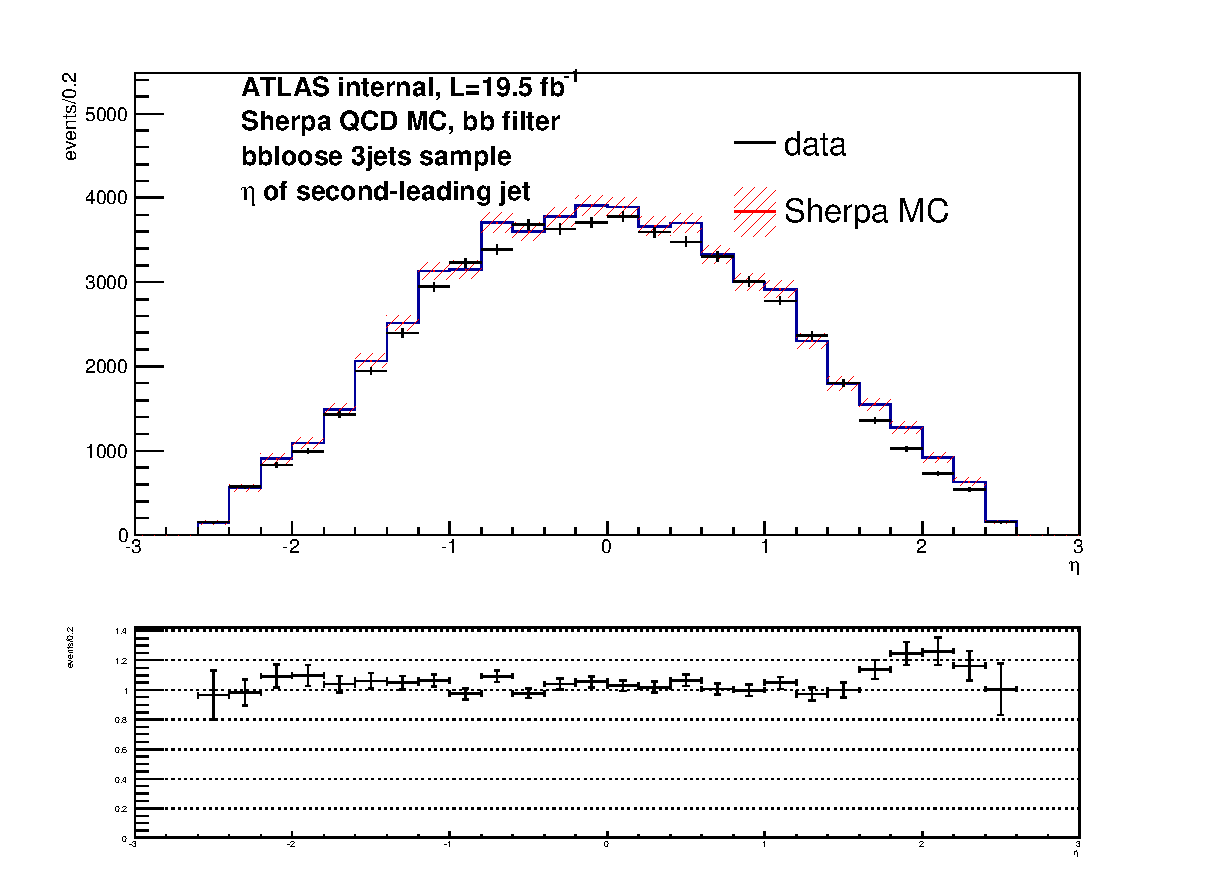
\includegraphics[width=\textwidth]{MonteCarlo/figures/eta1_bbloose_3jets.eps}\end{subfigure}
  \begin{subfigure}[$bbloose$ 4 jet category]{0.3\textwidth}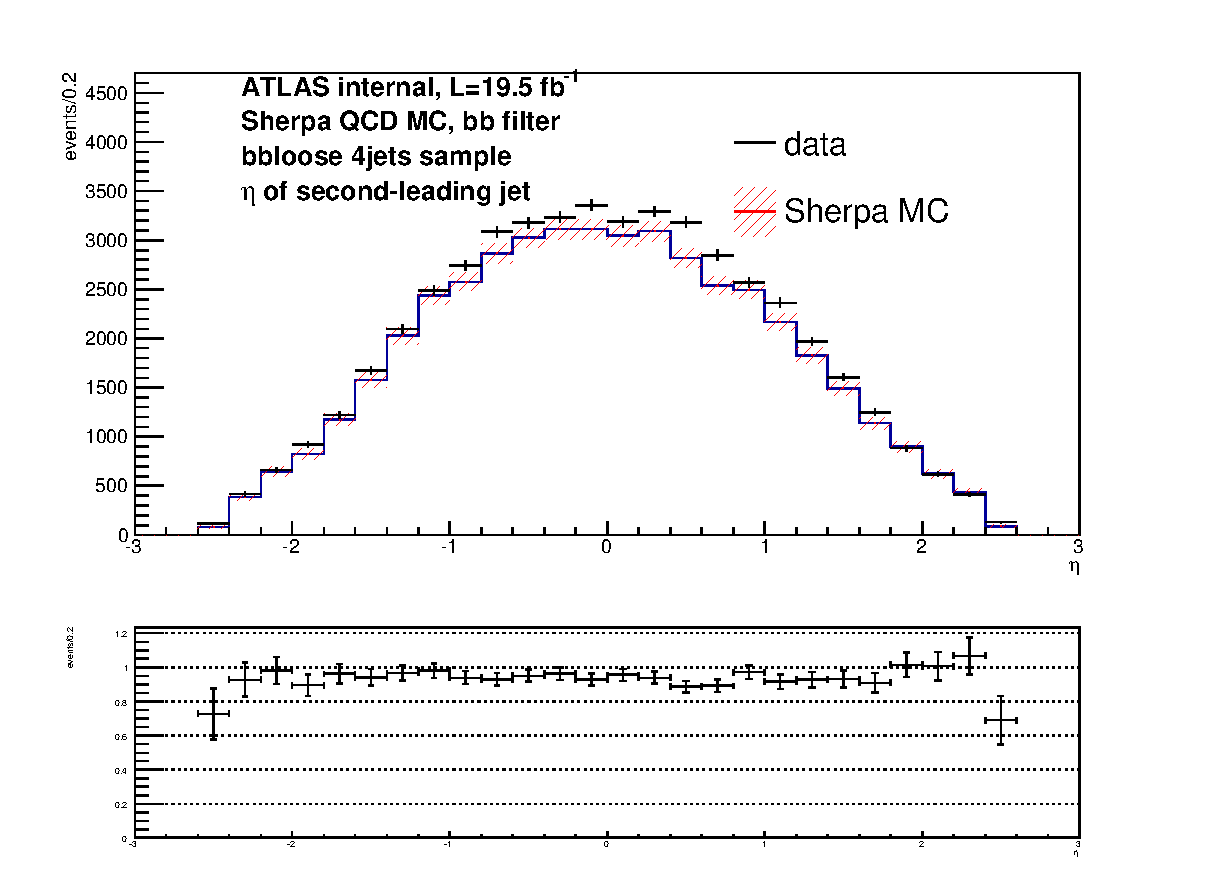
\includegraphics[width=\textwidth]{MonteCarlo/figures/eta1_bbloose_4jets.eps}\end{subfigure}
  \begin{subfigure}[$bbloose$ 5+ jet category]{0.3\textwidth}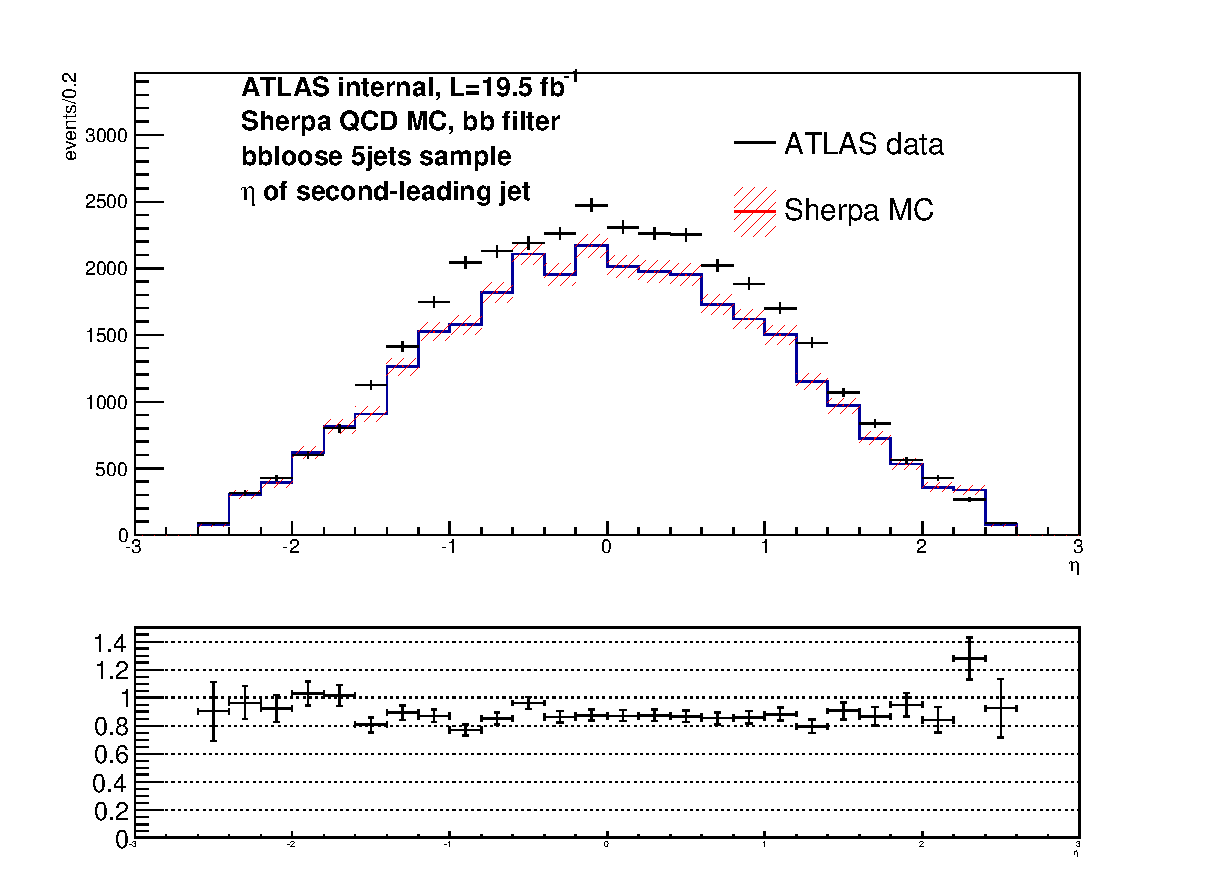
\includegraphics[width=\textwidth]{MonteCarlo/figures/eta1_bbloose_5jets.eps}\end{subfigure}
  \begin{subfigure}[$bbanti$ 3 jet category]{0.3\textwidth}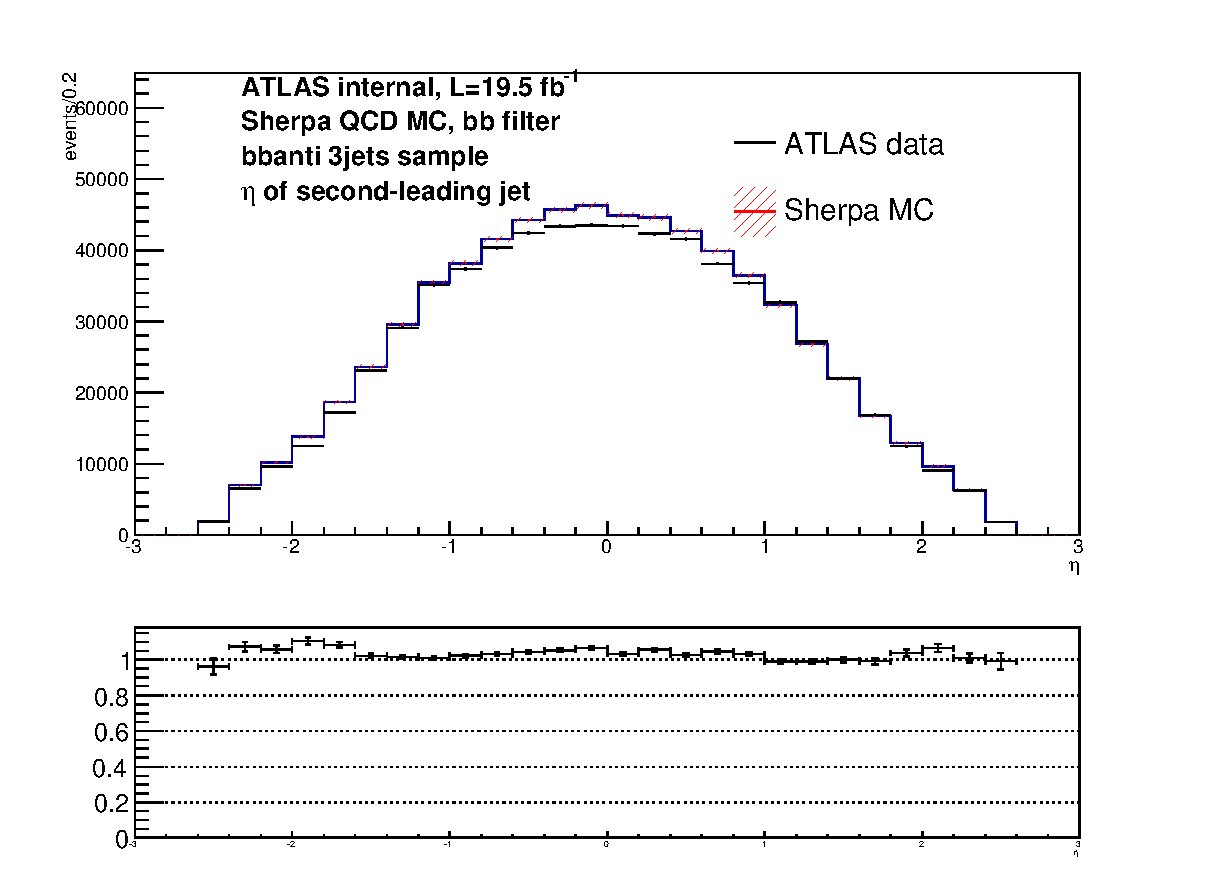
\includegraphics[width=\textwidth]{MonteCarlo/figures/eta1_bbanti_3jets.eps}\end{subfigure}
  \begin{subfigure}[$bbanti$ 4 jet category]{0.3\textwidth}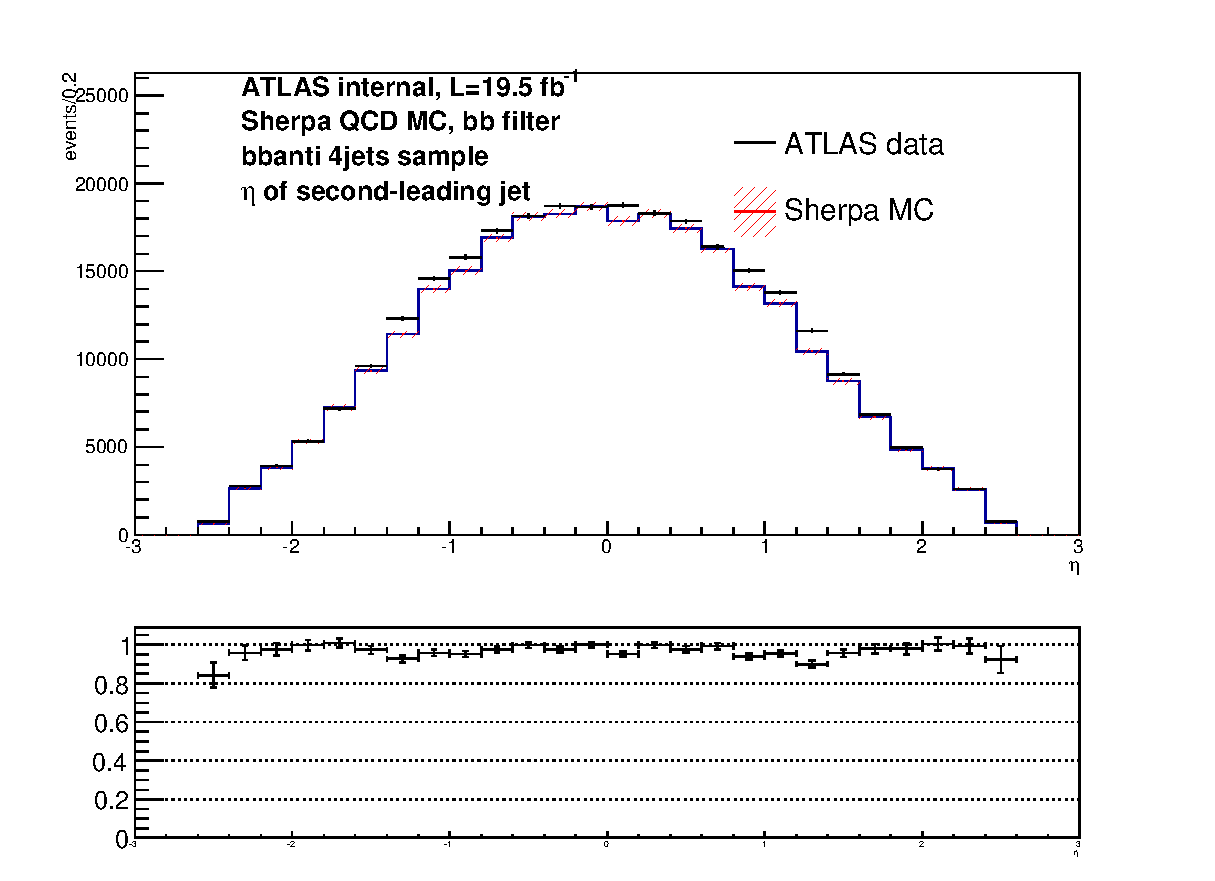
\includegraphics[width=\textwidth]{MonteCarlo/figures/eta1_bbanti_4jets.eps}\end{subfigure}
  \begin{subfigure}[$bbanti$ 5+ jet category]{0.3\textwidth}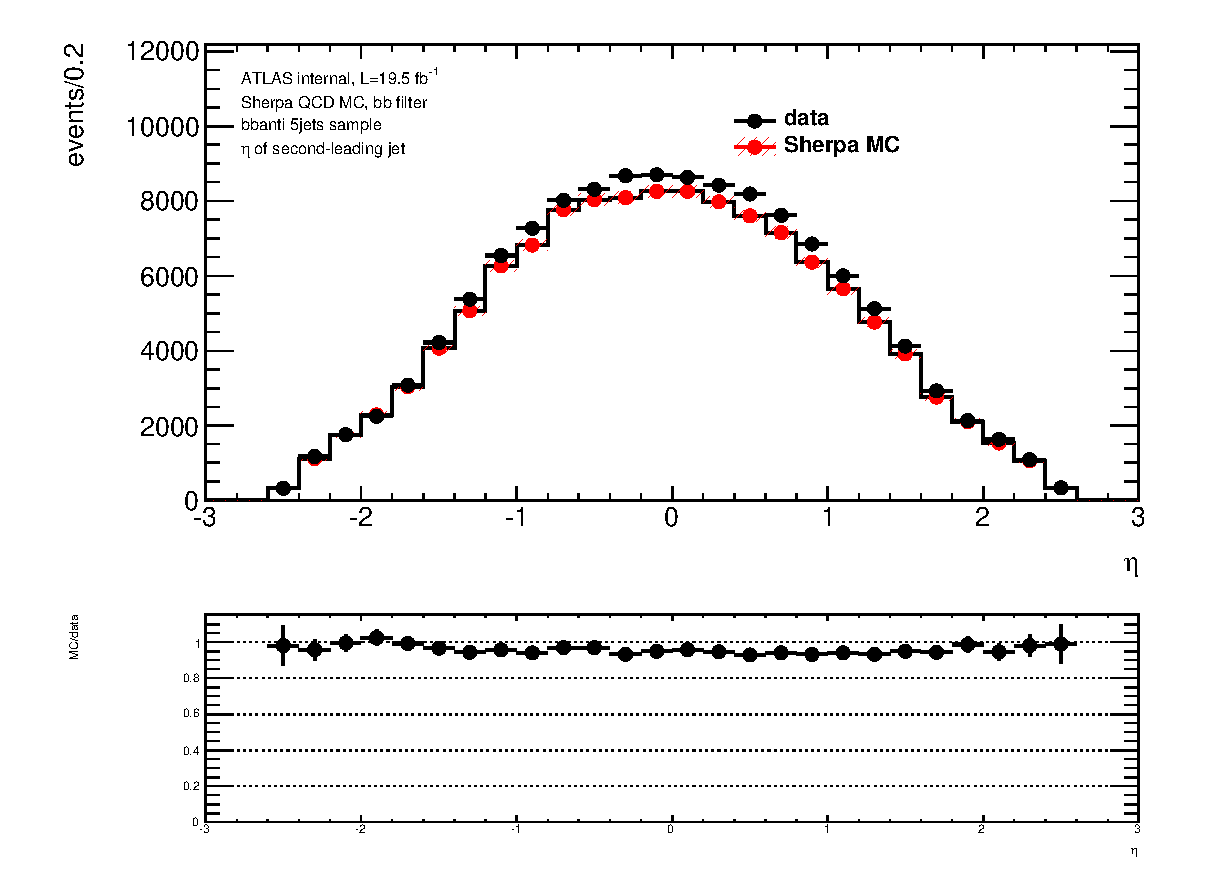
\includegraphics[width=\textwidth]{MonteCarlo/figures/eta1_bbanti_5jets.eps}\end{subfigure}
  \caption{The $\eta$ distributions for the second-leading jet, comparing bb QCD MC events to data.  The MC has been normalized
  to the same total number of events as the data (over the entire sample, not on a category-by-category basis)
  and the MC/data ratio is plotted in the lower subplots.  The errors on the MC are statistical only.
  \label{fig:bb_qcd_mc_eta1}}
    \end{center}
\end{figure}






\begin{figure}[phtb!]
  \begin{center}
  \begin{subfigure}[$bbb$ 3 jet category]{0.3\textwidth}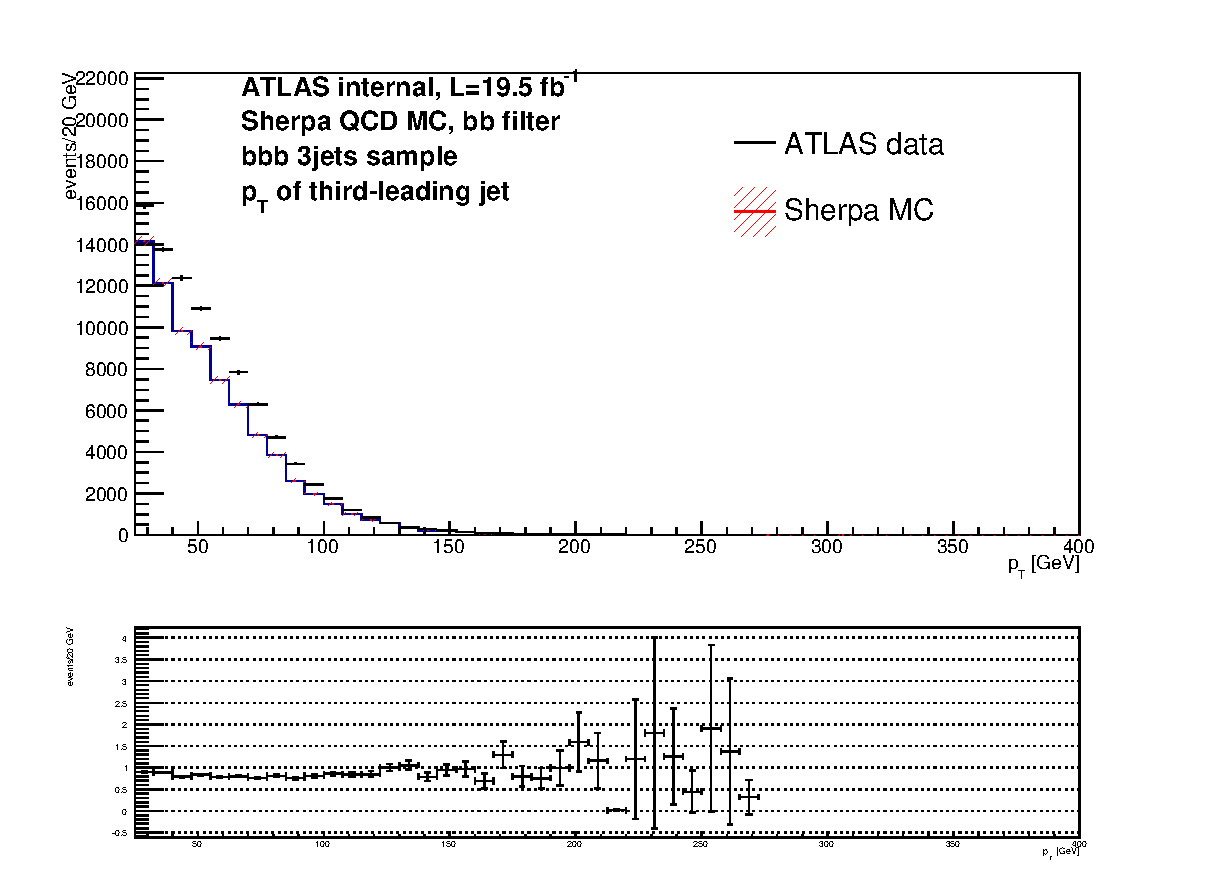
\includegraphics[width=\textwidth]{MonteCarlo/figures/pt2_bbb_3jets.eps}\end{subfigure}
  \begin{subfigure}[$bbb$ 4 jet category]{0.3\textwidth}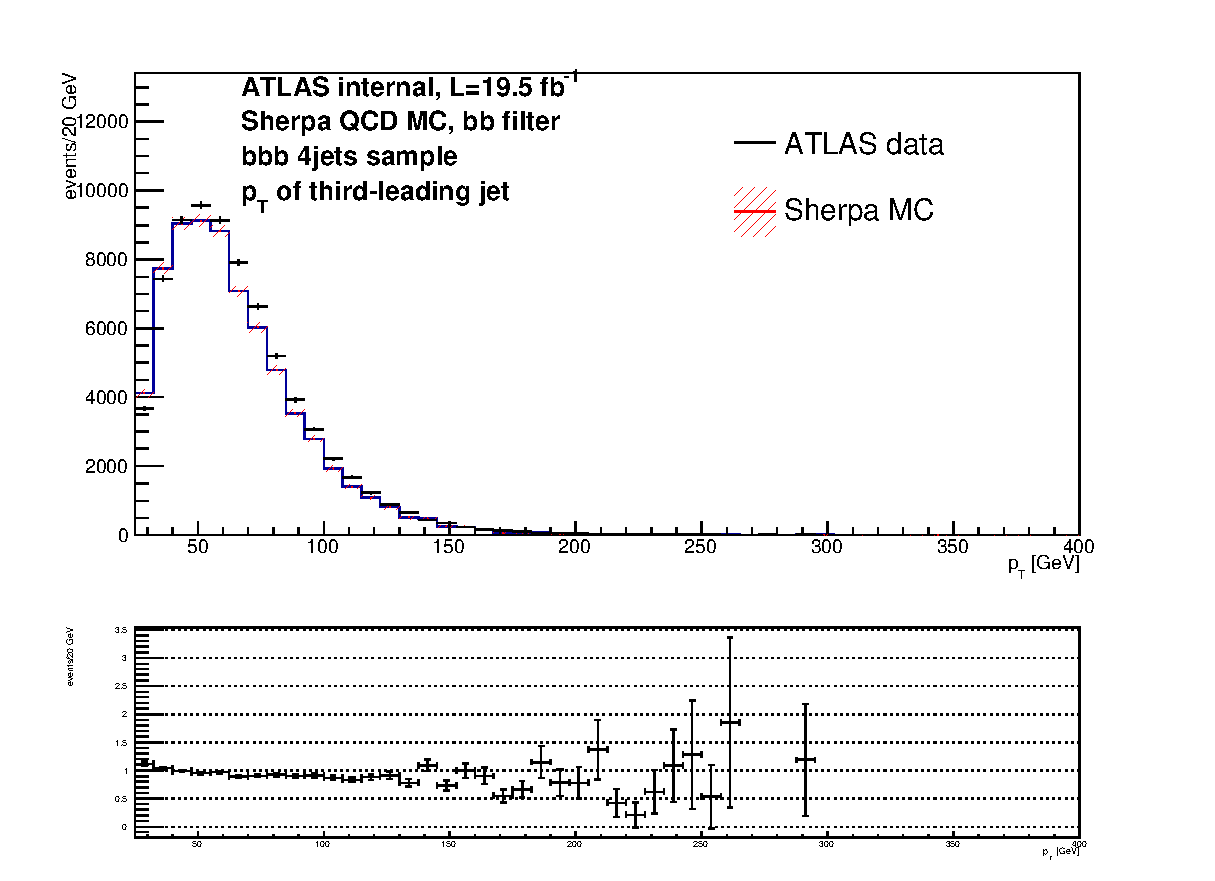
\includegraphics[width=\textwidth]{MonteCarlo/figures/pt2_bbb_4jets.eps}\end{subfigure}
  \begin{subfigure}[$bbb$ 5+ jet category]{0.3\textwidth}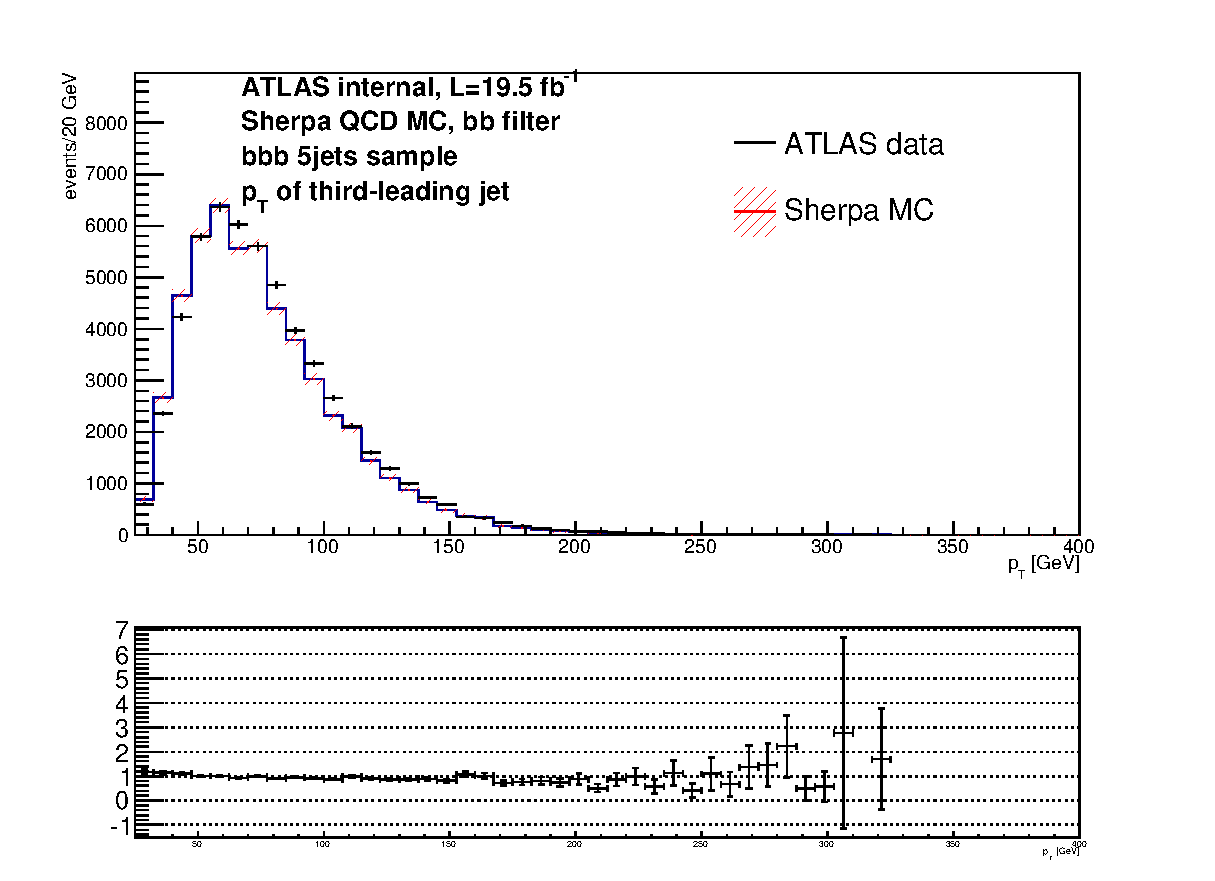
\includegraphics[width=\textwidth]{MonteCarlo/figures/pt2_bbb_5jets.eps}\end{subfigure}
  \begin{subfigure}[$bbloose$ 3 jet category]{0.3\textwidth}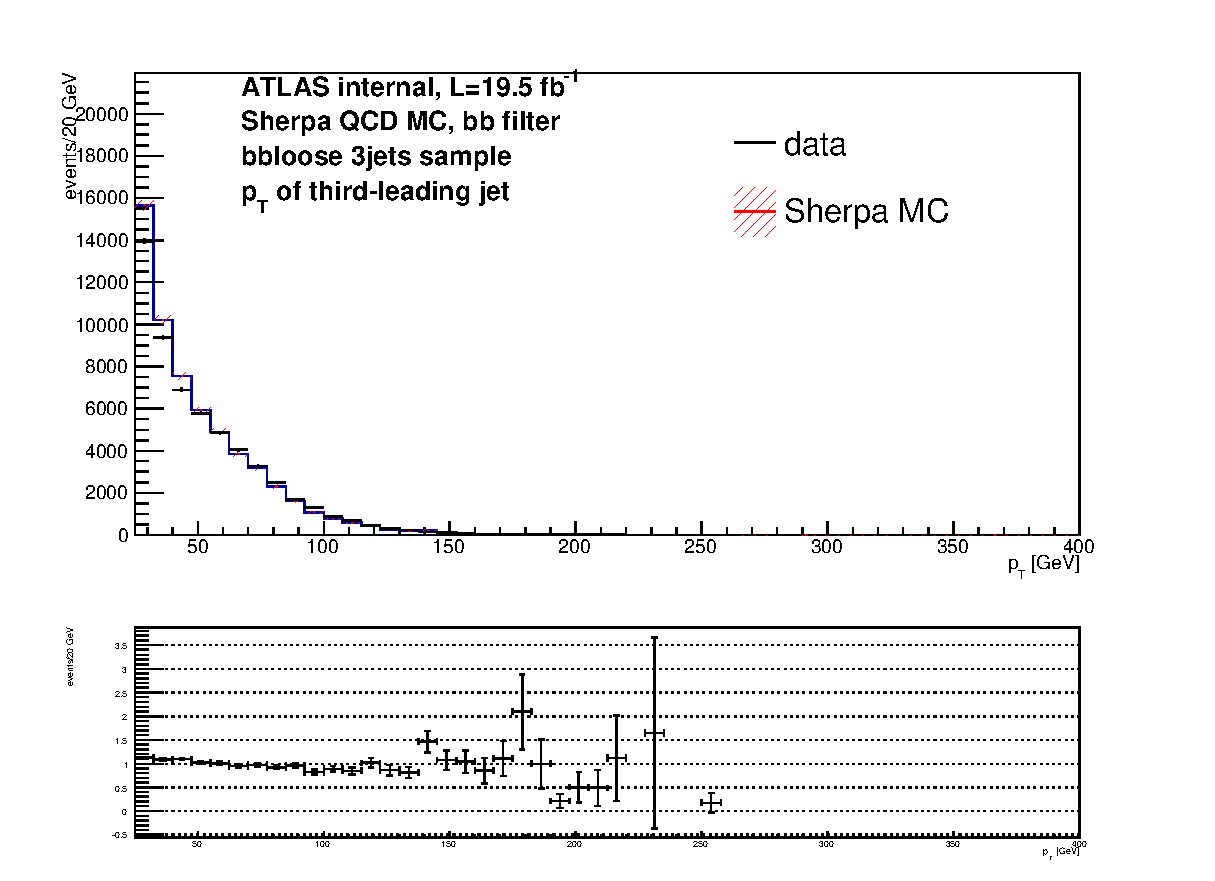
\includegraphics[width=\textwidth]{MonteCarlo/figures/pt2_bbloose_3jets.eps}\end{subfigure}
  \begin{subfigure}[$bbloose$ 4 jet category]{0.3\textwidth}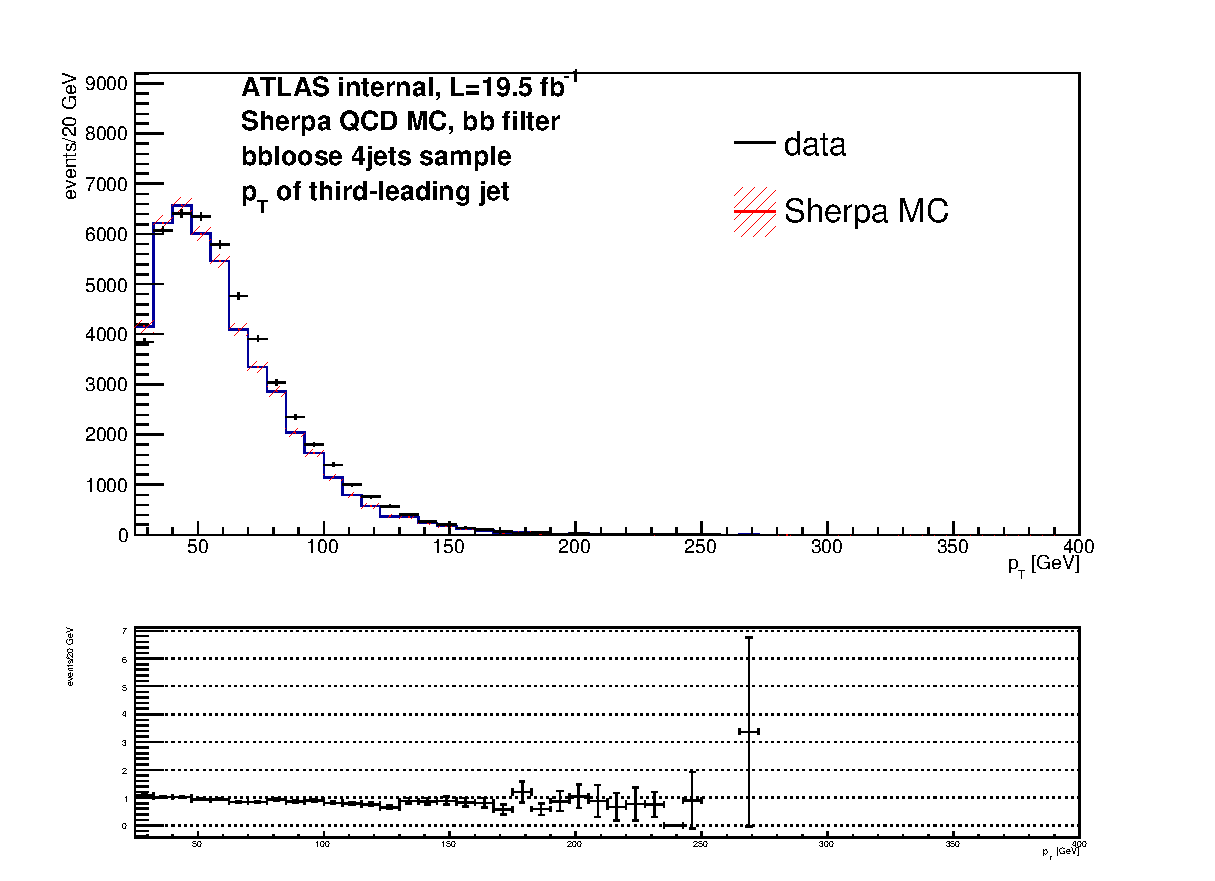
\includegraphics[width=\textwidth]{MonteCarlo/figures/pt2_bbloose_4jets.eps}\end{subfigure}
  \begin{subfigure}[$bbloose$ 5+ jet category]{0.3\textwidth}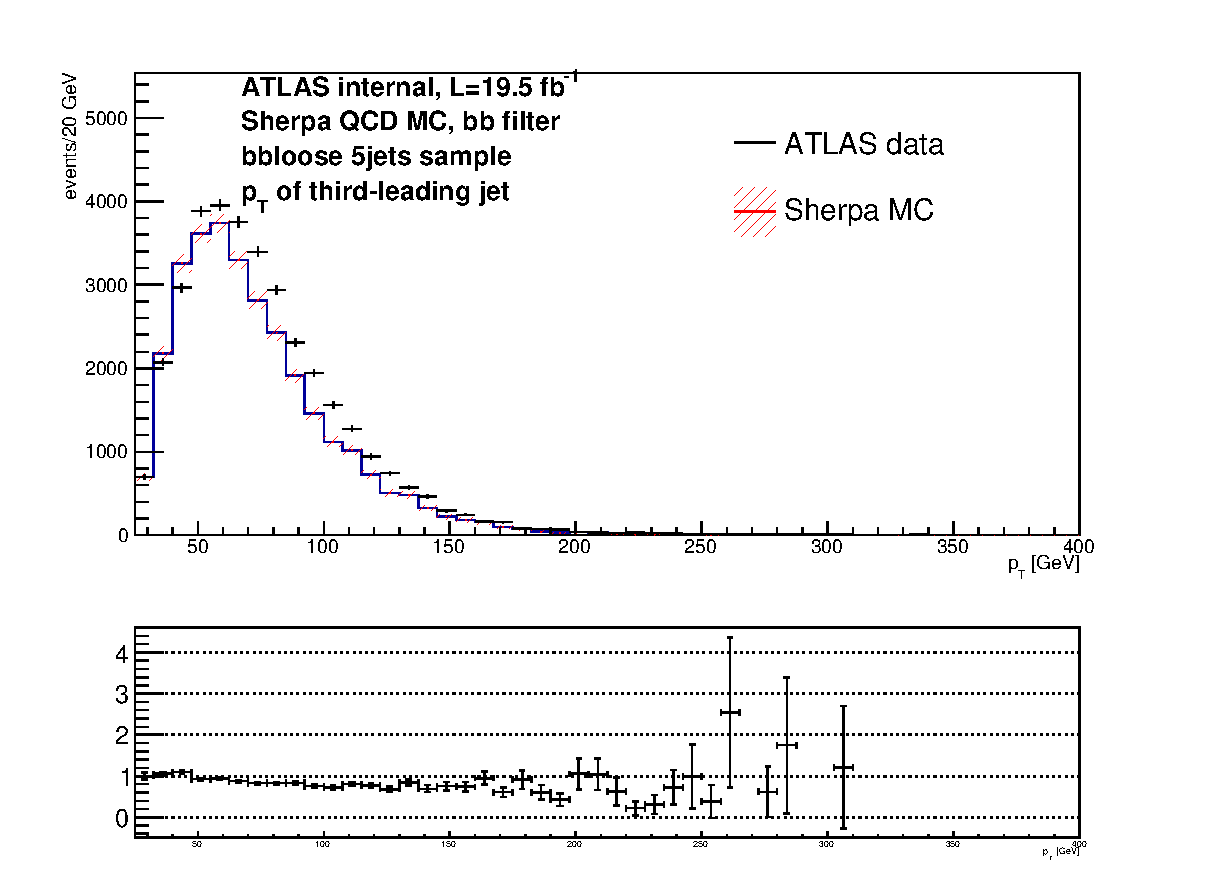
\includegraphics[width=\textwidth]{MonteCarlo/figures/pt2_bbloose_5jets.eps}\end{subfigure}
  \begin{subfigure}[$bbanti$ 3 jet category]{0.3\textwidth}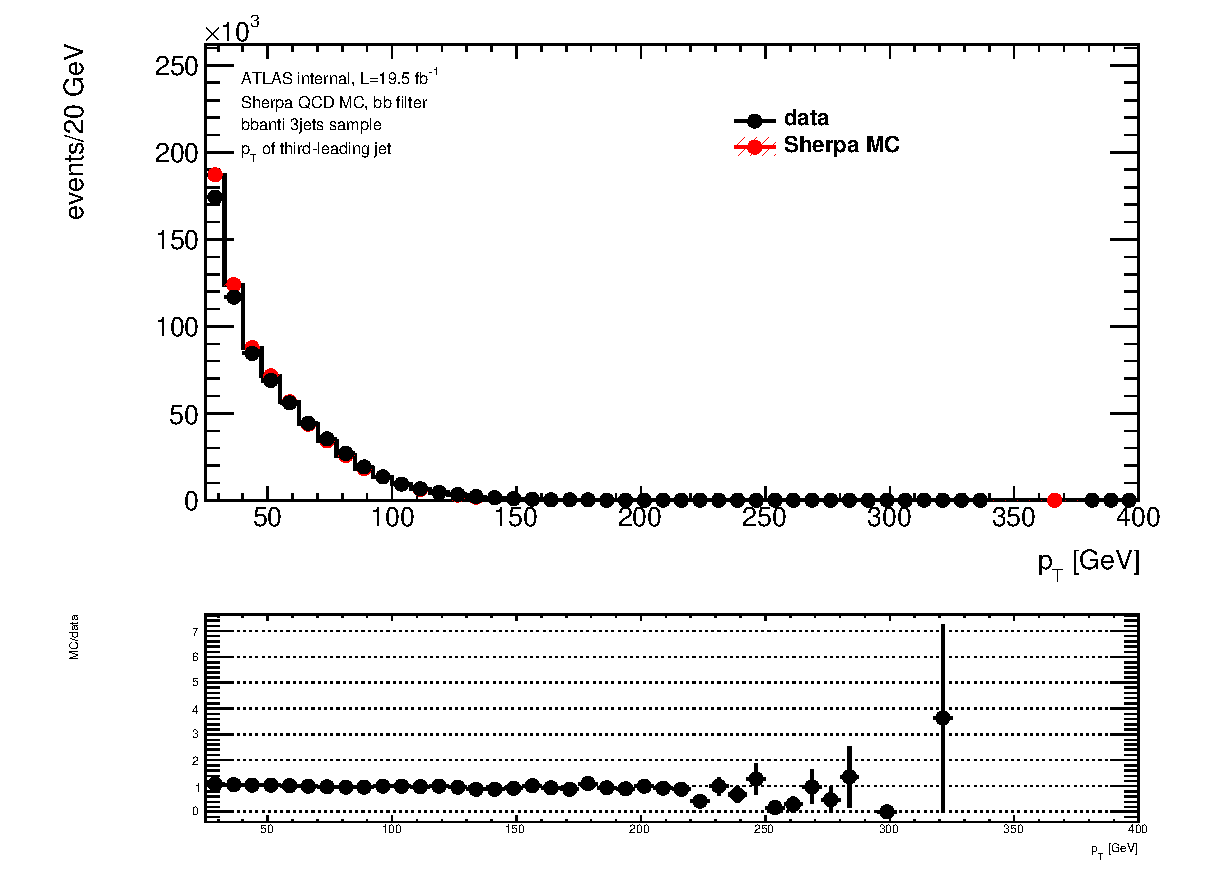
\includegraphics[width=\textwidth]{MonteCarlo/figures/pt2_bbanti_3jets.eps}\end{subfigure}
  \begin{subfigure}[$bbanti$ 4 jet category]{0.3\textwidth}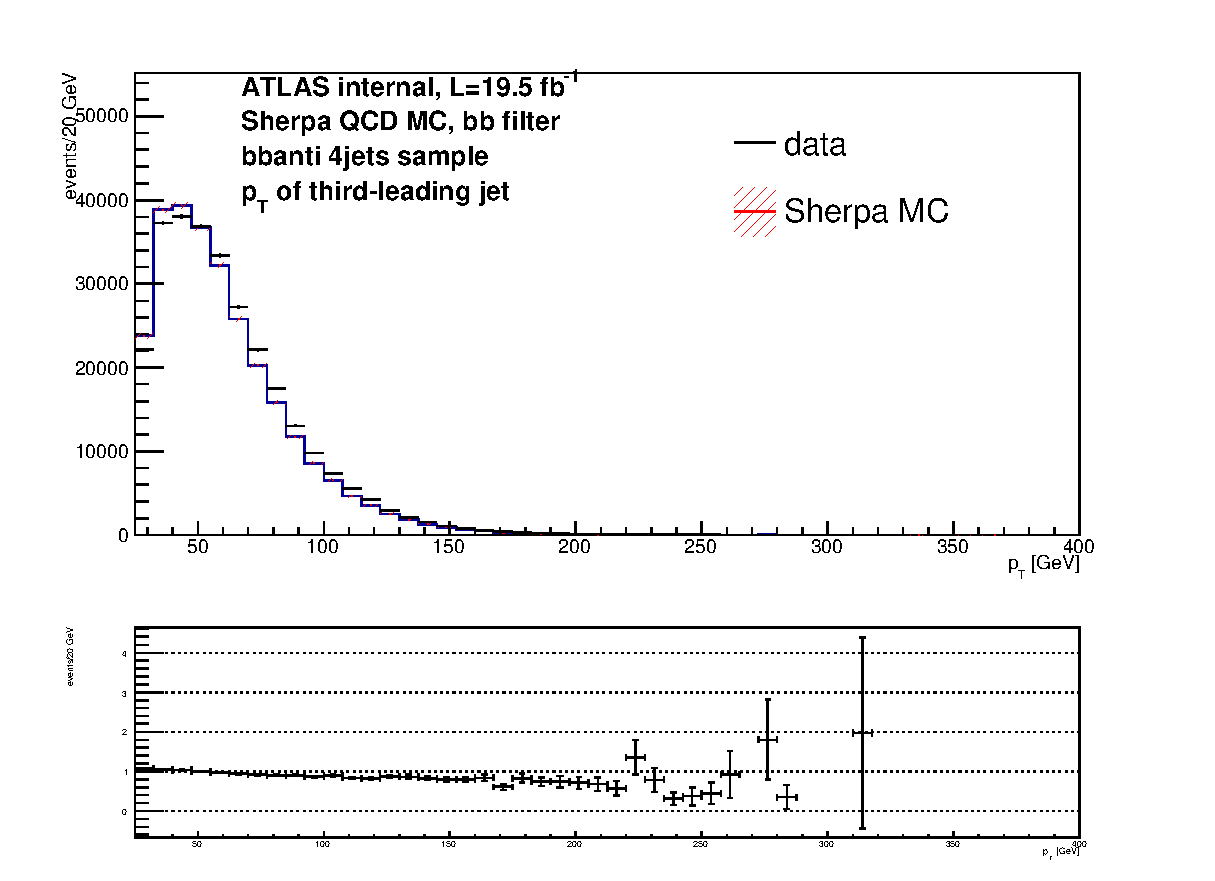
\includegraphics[width=\textwidth]{MonteCarlo/figures/pt2_bbanti_4jets.eps}\end{subfigure}
  \begin{subfigure}[$bbanti$ 5+ jet category]{0.3\textwidth}\includegraphics[width=\textwidth]{MonteCarlo/figures/pt2_bbanti_5jets.eps}\end{subfigure}
  \caption{The $p_T$ distributions for the third-leading jet, comparing bb QCD MC events to data.  The MC has been normalized
  to the same total number of events as the data (over the entire sample, not on a category-by-category basis)
  and the MC/data ratio is plotted in the lower subplots.  The errors on the MC are statistical only.
  \label{fig:bb_qcd_mc_pt2}}
    \end{center}
\end{figure}



\begin{figure}[phtb!]
  \begin{center}
  \begin{subfigure}[$bbb$ 3 jet category]{0.3\textwidth}\includegraphics[width=\textwidth]{MonteCarlo/figures/eta2_bbb_3jets.eps}\end{subfigure}
  \begin{subfigure}[$bbb$ 4 jet category]{0.3\textwidth}\includegraphics[width=\textwidth]{MonteCarlo/figures/eta2_bbb_4jets.eps}\end{subfigure}
  \begin{subfigure}[$bbb$ 5+ jet category]{0.3\textwidth}\includegraphics[width=\textwidth]{MonteCarlo/figures/eta2_bbb_5jets.eps}\end{subfigure}
  \begin{subfigure}[$bbloose$ 3 jet category]{0.3\textwidth}\includegraphics[width=\textwidth]{MonteCarlo/figures/eta2_bbloose_3jets.eps}\end{subfigure}
  \begin{subfigure}[$bbloose$ 4 jet category]{0.3\textwidth}\includegraphics[width=\textwidth]{MonteCarlo/figures/eta2_bbloose_4jets.eps}\end{subfigure}
  \begin{subfigure}[$bbloose$ 5+ jet category]{0.3\textwidth}\includegraphics[width=\textwidth]{MonteCarlo/figures/eta2_bbloose_5jets.eps}\end{subfigure}
  \begin{subfigure}[$bbanti$ 3 jet category]{0.3\textwidth}\includegraphics[width=\textwidth]{MonteCarlo/figures/eta2_bbanti_3jets.eps}\end{subfigure}
  \begin{subfigure}[$bbanti$ 4 jet category]{0.3\textwidth}\includegraphics[width=\textwidth]{MonteCarlo/figures/eta2_bbanti_4jets.eps}\end{subfigure}
  \begin{subfigure}[$bbanti$ 5+ jet category]{0.3\textwidth}\includegraphics[width=\textwidth]{MonteCarlo/figures/eta2_bbanti_5jets.eps}\end{subfigure}
  \caption{The $\eta$ distributions for the third-leading jet, comparing bb QCD MC events to data.  The MC has been normalized
  to the same total number of events as the data (over the entire sample, not on a category-by-category basis)
  and the MC/data ratio is plotted in the lower subplots.  The errors on the MC are statistical only.
  \label{fig:bb_qcd_mc_eta2}}
    \end{center}
\end{figure}








\begin{figure}[phtb!]
  \begin{center}
  \begin{subfigure}[$BBB$ vs $BBC$, 3 jet category]{0.45\textwidth}\includegraphics[width=\textwidth]{MonteCarlo/figures/mbb_bbB_3jets_bbB_bbC.pdf}\end{subfigure}
  \begin{subfigure}[$BBB$ vs $BBL$, 3 jet category]{0.45\textwidth}\includegraphics[width=\textwidth]{MonteCarlo/figures/mbb_bbB_3jets_bbB_bbL.pdf}\end{subfigure}
  \caption{The $m_{bb}$ distributions in the 3 jet category, where the third jet in the event has been 
  truth-matched as bottom versus charm (left) or light (right).  The distributions have been normalized to 
  the same integral, and the lower subplots show the ratio of charm (light) to bottom.  Errors on the MC
  are statistical only.  There is no evidence from these distributions that the $m_{bb}$ of the leading
  2 jets in a QCD event is affected by the truth flavor of the third jet. 
  \label{fig:mbb_bb_qcd_mc}}
    \end{center}
\end{figure}








\begin{figure}[phtb!]
  \begin{center}
  \begin{subfigure}[$BBB$ vs $BBC$, 4 jet category]{0.45\textwidth}\includegraphics[width=\textwidth]{MonteCarlo/figures/mbb_bbB_4jets_bbB_bbC.pdf}\end{subfigure}
  \begin{subfigure}[$BBB$ vs $BBL$, 4 jet category]{0.45\textwidth}\includegraphics[width=\textwidth]{MonteCarlo/figures/mbb_bbB_4jets_bbB_bbL.pdf}\end{subfigure}
  \caption{The $m_{bb}$ distributions in the 4 jet category, where the third jet in the event has been 
  truth-matched as bottom versus charm (left) or light (right).  The distributions have been normalized to 
  the same integral, and the lower subplots show the ratio of charm (light) to bottom.  Errors on the MC
  are statistical only.  There is no evidence from these distributions that the $m_{bb}$ of the leading
  2 jets in a QCD event is affected by the truth flavor of the third jet. 
  \label{fig:mbb_bb_qcd_mc}}
    \end{center}
\end{figure}






\begin{figure}[phtb!]
  \begin{center}
  \begin{subfigure}[$BBB$ vs $BBC$, 5+ jet category]{0.45\textwidth}\includegraphics[width=\textwidth]{MonteCarlo/figures/mbb_bbB_5jets_bbB_bbC.pdf}\end{subfigure}
  \begin{subfigure}[$BBB$ vs $BBL$, 5+ jet category]{0.45\textwidth}\includegraphics[width=\textwidth]{MonteCarlo/figures/mbb_bbB_5jets_bbB_bbL.pdf}\end{subfigure}
  \caption{The $m_{bb}$ distributions in the 5 or more jet category, where the third jet in the event has been 
  truth-matched as bottom versus charm (left) or light (right).  The distributions have been normalized to 
  the same integral, and the lower subplots show the ratio of charm (light) to bottom.  Errors on the MC
  are statistical only.  There is no evidence from these distributions that the $m_{bb}$ of the leading
  2 jets in a QCD event is affected by the truth flavor of the third jet. 
  \label{fig:mbb_bb_qcd_mc}}
    \end{center}
\end{figure}










%-----------------------------------------------                     



%\subsection{Top Background}
%Top-antitop pairs decaying all-hadronically is the largest non-QCD background.  The sample generated
%to model this background is generated in Powheg and Pythia, with Tauola and Photos also used for
%handling tau leptons and photons.  In practice, $t\bar{t}$ is a minor background, both because
%of its small cross section relative to QCD and because in the high mass ranges most relevant for
%this search, it does not show any sigificant structure or $m_{bb}$ shape differences depending
%on the flavor of the third jet.
%
%
%\begin{table}
%%    \begin{center}
%   \caption{Parameters of the $t\bar{t}$ MC sample used in this analysis. \label{tab:ttbar_params} }
%    \begin{tabular}{ c c c c }
%    Dataset ID & Cross Section [nb] & Filter Efficiency & N Events \\
%    117050     & 0.21085        & 0.54298    & 99930891 \\
%    \end{tabular}
%    \end{center}
%\end{table}

%--------------------------------------------------------






